\NeedsTeXFormat{LaTeX2e}[1995/12/01]
%%
%% This is file `ubcsample.tex',
%% generated with the docstrip utility.
%
% The original source files were:
%
% ubcthesis.dtx  (with options: `ubcsampletex')
%% 
%% This file was generated from the ubcthesis package.
%% --------------------------------------------------------------
%% 
%% Copyright (C) 2001
%% Michael McNeil Forbes
%% mforbes@alum.mit.edu
%% 
%% This file may be distributed and/or modified under the
%% conditions of the LaTeX Project Public License, either version 1.2
%% of this license or (at your option) any later version.
%% The latest version of this license is in
%%    http://www.latex-project.org/lppl.txt
%% and version 1.2 or later is part of all distributions of LaTeX
%% version 1999/12/01 or later.
%% 
%% This program is distributed in the hope that it will be useful,
%% but WITHOUT ANY WARRANTY; without even the implied warranty of
%% MERCHANTABILITY or FITNESS FOR A PARTICULAR PURPOSE.  See the
%% LaTeX Project Public License for more details.
%% 
%% This program consists of the files ubcthesis.dtx, ubcthesis.ins, and
%% the sample figures fig.eps and fig.fig.
%% 
%% This file may be modified and used as a base for your thesis without
%% including the licence agreement as long as the content (i.e. textual
%% body) of the file is completely rewritten. You must, however, change
%% the name of the file.
%% 
%% This file may only be distributed together with a copy of this
%% program. You may, however, distribute this program without generated
%% files such as this one.
%% 


% This Sample thesis requires \LaTeX2e
\NeedsTeXFormat{LaTeX2e}[1995/12/01]
%\ProvidesFile{ubcsample.tex}[2015/05/31 v1.72 ^^J
% University of British Columbia Sample Thesis]
% This is the \documentclass[]{} command.  The manditory argument
% specifies the "flavour" of thesis (ubcthesis for UBC).  The
% optional arguments (in []) specify options that affect how the
% thesis is displayed.  Please see the ubcthesis documentation for
% details about the options.
\documentclass[msc,oneside]{ubcthesis}
%\usepackage[pass,paperwidth=8.5in,paperheight=11in]{geometry}
\usepackage[
paperwidth=8.5in,
paperheight=11in,
% other options: a3paper, a5paper, etc
left=3.2cm,
right=2.5cm,
top=2.5cm,
bottom=2.5cm,
% use vmargin=2cm to make vertical margins equal to 2cm.
% us  hmargin=3cm to make horizontal margins equal to 3cm.
% use margin=3cm to make all margins  equal to 3cm.
]
{geometry}
%\pdfpageheight=11in
%\pdfpagewidth=8.5in
%
% To compile this sample thesis, issue the following commands:
% latex ubcsample
% bibtex ubcsample
% latex ubcsample
% latex ubcsample
% latex ubcsample
%
% To view use xdvi (on unix systems):
% xdvi ubcsample.dvi
%
% To make a postscript file, use dvips:
% dvips -o ubcsample.ps ubcsample.dvi
%
% To view the postscript file, use ghostview or gv (on unix systems):
% gv ubcsample.ps
%
%************************************************
% Optional packages.
%
% The use of these packages is optional, but they provide various
% tools for more flexible formating.  The sample thesis uses these,
% but if you remove the example code, you should be able to exclude
% these packages.  Only standard packages have been described here;
% they should be installed with any complete LaTeX instalation, but
% if not, you can find them at the Comprehensive TeX Archive Network
% (CTAN): http://www.ctan.org/
%

%******** afterpage ***************************
% This package allows you to issue commands at the end of the current
% page.  A good use for this is to use the command
% \afterpage{\clearpage} right after a figure.  This will cause the
% figure to be inserted on the page following the current one (or on
% the current page if it will fit) but will not break the page in the
% middle.
\usepackage{afterpage}
\usepackage{xcolor}
%******** float *********************************
% This package allows you to customize the style of
% "floats"---floating objects such as figures and tables.  In
% addition, it allows you to define additional floating objects which
% may be included in a list similar to that produces by \listoftables
% and \listoffigures.  Common uses include introducing floats for
% programs and other code bits in Compute Science and Chemical Schema.
\usepackage{float}
\usepackage{amsmath,bm}
\usepackage{tikz}
\usepackage{quantikz}
\usepackage{tabularray}
\usepackage{dsfont}
\usetikzlibrary{shapes.geometric}
\usetikzlibrary{arrows.meta} % For arrow tips
\usepackage{xcolor} % For colors
\definecolor{lightblue}{RGB}{173,216,230} % Define light blue
%******** tocloft *******************************
% This package allows you to customize and define custom lists such
% as a list of programs or Chemical Scheme.  Note: if you use the
% subfigure package, you must specify that you do as an option here.
% The title option uses the default formatting.  We do not use this
% here as the default formatting is acceptable.  Use the float
% package instead unless you need the extra formatting control
% provided by tocloft.
%\usepackage[subfigure, titles]{tocloft}

%******** alltt *********************************
% The alltt package allows you to include files and have them
% formatted in a verbatim fashion.  This is useful for including
% source code from an additional file.
%\usepackage{alltt}

%******** listings ******************************
% The listings package may be used to include chunks of source code
% and has facilities for pretty-printing many languages.
%\usepackage{listings}

%******** longtable *****************************
% The longtable package allows you to define tables that span
% multiple pages.



\usepackage{longtable}

%******** graphics and graphicx *****************
% This allows you to include encapsulated postscript files.  If you
% don't have this, comment the \includegraphics{} line following the
% comment "%includegraphics" later in this file.
\usepackage{graphicx}

%******** subfigure *****************************
% The subfigure package allows you to include multiple figures and
% captions within a single figure environment.
%\usepackage{subfigure}

%******** here **********************************
% The here package gives you more control over the placement of
% figures and tables.  In particular, you can specify the placement
% "H" which means "Put the figure here" rather than [h] which means
% "I would suggest that you put the figure here if you think it looks
% good."
%\usepackage{here}

%******** pdflscape ********************************
% This allows you to include landscape layout pages by using the
% |landscape| environment.  The use of |pdflscape| is preferred over
% the standard |lscape| package because it automatically rotates the
% page in the pdf file for easier reading.  (Thanks to Joseph Shea
% for pointing this out.)
\usepackage{pdflscape}
\usepackage{pdfpages}

%******** natbib ********************************
% This is a very nice package for bibliographies.  It includes options
% for sorting and compressing bibliographic entries.
\usepackage[numbers,sort&compress]{natbib}
%\usepackage{natbib}   % omit 'round' option if you prefer square brackets

%\usepackage{hyperref}
\usepackage[unicode=true,
colorlinks=true,
linktocpage,
linkbordercolor={0.5 0.5 1},
citebordercolor={0.5 1 0.5},
linkcolor=blue]{hyperref}


\usepackage[nameinlink]{cleveref}


% for clever referencing, i.e. references equations as e.g.: eq. (1.1), particularly useful together with hyperref (which is automatically loaded by jcappub)

%******** psfrag ******************************
% This allows you to replace text in postscript pictures with formated
% latex text.  This allows you to use math in graph labels
% etc. Uncomment the psfrag lines following the "%psfrag" comment
% later in this file if you don't have this package.  The replacements
% will only be visible in the final postscript file: they will be
% listed in the .dvi file but not performed.
%\usepackage{psfrag}
%\usepackage[margin=0.5in]{geometry}
%******** hyperref *****************************
% Please read the manual:
% http://www.tug.org/applications/hyperref/manual.html
%
% This adds hyperlinks to your document: with the right viewers (later
% versions of xdvi, acrobat with pdftex, latex2html etc.) this will
% make your equation, figure, citation references etc. hyperlinks so
% that you can click on them.  Also, your table of contents will be
% able to take you to the appropriate sections.  In the viewers that
% support this, the links often appear with an underscore.  This
% underscore will not appear in printed versions.
%
% Note: if you do not use the hypertex option, then the dvips driver
% may be loaded by default.  This will cause the entries in the list
% of figures and list of tables to be on a single line because dvips
% does not deal with hyperlinks on broken lines properly.
%
% NOTE: HYPERREF is sensitive to the ORDER in which it is LOADED.
% For example, it must be loaded AFTER natbib but BEFORE newly
% defined float environments.  See the README file with the hyperref
% for some help with this.  If you have some very obscure errors, try
% first disabling hyperref.  If that fixes the problem, try various
% orderings.
%
% Note also that there is a bug with versions before 2003/11/30
% v6.74m that cause the float package to not function correctly.
% Please ensure you have a current version of this package.  A
% warning will be issued if you leave the date below but do not have
% a current version installed.
%
% Some notes on options: depending on how you build your files, you
% may need to choose the appropriate option (such as [pdftex]) for the
% backend driver (see the hyperref manual for a complete list).  Also,
% the default here is to make links from the page numbers in the table
% of contents and lists of figures etc.  There are other options:
% excluding the [linktocpage] option will make the entire text a
% hyperref, but for some backends will prevent the text from wrapping
% which can look terrible.  There is a [breaklinks=true] option that
% will be set if the backend supports (dvipdfm for example supports
% it but does not work with psfrag.)
%
% Finally, there are many options for choosing the colours of the
% links.  These will be included by default in future versions but
% you should probably consider changing some now for the electronic
% version of your thesis.
%\usepackage[unicode=true,
%  linktocpage,
%  linkbordercolor={0.5 0.5 1},
%  citebordercolor={0.5 1 0.5},
%  linkcolor=blue]{hyperref}

% If you would like to compile this sample thesis without the
% hyperref package, then you will need to comment out the previous
% \usepackage command and uncomment the following command which will
% put the URL's in a typewriter font but not link them.
%\newcommand\url[1]{\texttt{#1}}

%******** setspace *******************************
% The setspace package allows you to manually set the spacing of the
% file.  UBC may require 1.5 spacing for microfilming of theses.  In
% this case you may obtain this by including this package and issuing
% one of the following commands:
%\usepackage{setspace}
%\singlespacing
%\onehalfspacing
%\doublespacing

% These commands are optional.  The defaults are shown.  You only
% need to include them if you need a different value
\institution{The University Of British Columbia}

% If you are at the Okanagan campus, then you should specify these
% instead.
%\faculty{The College of Graduate Studies}
%\institutionaddress{Okanagan}
\faculty{The Faculty of Science}
\institutionaddress{Vancouver}

% You can issue as many of these as you have...
%\previousdegree{B.Sc., University of British Columbia, year}
%\previousdegree{M.Sc., The University of British Columbia, 2022}
%\previousdegree{Ph.D., Massachusetts Institute of Technology, 2005}

% You can override the option setting here.
\degreetitle{Bachelor of Science}

% These commands are required.
\title{A Quantum Algorithm for the Bottleneck Travelling Salesman Problem}
%\subtitle{With a Subtitle}
\author{Raveel Tejani}
%\copyrightyear{2000}
\submitdate{\monthname\ \number\year} % The "\ " is required after
% \monthname to prevent the
% command from eating the space.
\program{Physics}

% These commands are presently not required for UBC theses as the
% advisor's name and title are not presently required anywhere.
%\advisor{Ariel R.~Zhitnitsky}
%\advisortitle{Professor of Physics}

% One might want to override the format of the section and chapter
% numbers.  This shows you how to do it.  Note that the current
% format is acceptable for submission to the FoGS: If you wish to modify
% these, you should check with the FoGS explicity. prior to making
% the modifications.
\renewcommand\thepart         {\Roman{part}}
\renewcommand\thechapter      {\arabic{chapter}}
\renewcommand\thesection      {\thechapter.\arabic{section}}
\renewcommand\thesubsection   {\thesection.\arabic{subsection}}
\renewcommand\thesubsubsection{\thesubsection.\arabic{subsubsection}}
\renewcommand\theparagraph    {\thesubsubsection.\arabic{paragraph}}
\renewcommand\thesubparagraph {\theparagraph.\arabic{subparagraph}}

\setcounter{tocdepth}{2}
\setcounter{secnumdepth}{2}
%\newcommand{\arefe}[1]{{\textcolor{cyan}{#1}}}
% Here is an example of a "Program" environment defined with the
% "float" package.  The list of programs will be stored in the file
% ubcsample.lop and the numbering will start with the chapter
% number.  The style will be "ruled".
\floatstyle{ruled}
\newfloat{Program}{htbp}{lop}[chapter]






%%%%%%%%%%%%%%%%%%%%%%%%%%%%%%%%%%%%%%%%%%%%%%%%%%%%%%%%%%%%
%EVERTYTHING FOR JUPYTER NOTEBOOK%%%%%




%%%%%%%%%%%%%%%%%%%%%%%%%%%%%%%%%%%%%%%%%%%%%%%%%%%%%%%%%%%%%
% Here is the start of the document.
\begin{document}
	
	
	%% This starts numbering in Roman numerals as required for the thesis
	%% style and is mandatory.
	\frontmatter
	
	%%% The order of the following components should be preserved.  The order
	%%% listed here is the order currently required by FoGS:        \\
	%%% Title (Mandatory)                                           \\
	%%% Preface (Manditory if any collaborator contributions)       \\
	%%% Abstract (Mandatory)                                        \\
	%%% List of Contents, Tables, Figures, etc. (As appropriate)    \\
	%%% Acknowledgements (Optional)                                 \\
	%%% Dedication (Optional)                                       \\
	
	\maketitle                      %% Mandatory
	
	%\clearpage
	
	%%%THESIS APPROVAL PAGE - REQUIRED AS PART OF YOUR COMPLETED THESIS
	
	%%%%%%% UBC FoGPS Requires the following statements at the beginning of the thesis. There is a (separate) thesis approval form that has to be signed and dated by the same individuals listed here as approving the thesis. You will have to get ensure that your department submits that approval form before you will be able to create an account and upload your thesis onto ciRCle. 
	%\noindent
	%The following individuals certify that they have read, and recommend to the Faculty of Graduate and Postdoctoral Studies for acceptance, the thesis entitled:
	
	%\bigskip\noindent
	%\textbf{Title}
	
	
	
	%\bigskip\noindent
	%submitted by 
	%\textbf{Author}
	%in partial fulfillment of the requirements for
	%the degree of 
	%\textbf{program}
	%\bigskip\noindent
	%in	\textbf{Physics}
	
	
	%\bigskip\noindent
	%\textbf{[Include titles, departments, and universities, or titles and organizations. Remember to remove ALL material in square brackets [  ] before adding the page to your thesis.] Modify the examining committee to adapt to your case.}
	
	%\bigskip\noindent
	%\textbf{Examining Committee:}
	
	%\bigskip\noindent
	%Supervisor: 
	
	%\bigskip\noindent
	%Co-supervisor: \hrulefill
	
	%\bigskip\noindent
	%Supervisory Committee Member: \hrulefill
	
	%\bigskip\noindent
	%Additional Examiner: 
	
	%\bigskip\noindent
	%Additional Supervisory Committee Members: 
	
	%\bigskip\noindent
	%Supervisory Committee Member:\hrulefill
	
	
	
	
	
	
	
	\clearpage
	\begin{abstract}                %% Mandatory -  maximum 350 words
%		The \texttt{genthesis.cls} \LaTeX{} class file and accompanying
%		documents, such as this sample thesis, are distributed in the hope
%		that it will be useful but without any warranty (without even the
%		implied warranty of fitness for a particular purpose).  For a
%		description of this file's purpose, and instructions on its use, see
%		below.
%		
		%We present  a constraint and full solution to the bottleneck travelling salesman problem based on the quantum phase estimation algorithm.
		
		\textbf{chapter not complete.}
		
		
	\end{abstract}
	
%	\chapter{Lay Summary}
%	
%	%[Required, Maximum 150 words]
%	
%	%This is a simple summary of your thesis, written so that members of the public will get some idea about what you have done.
%	
%	%Full-sky simulations of the foreground radiation of the cosmic microwave background are computationally expensive and it is challenging to measure if they can replicate the same statistical properties as the real data. 
%	%In this thesis, I advocate for the use of a method called the ``hierarchical wavelet coefficients" for characterizing non-Gaussianities in a spherical field. This method is also known as the ``wavelet scattering transform" method and so far it has been mostly used for analysing flat (cutsky) maps. I demonstrate that the full-sky implementation introduced in this thesis is also capable of characterizing non-Gaussianities using a small set of coefficients.  
%	
%	%The algorithm for this method is based on the  \textsc{Healpy} package. 
%	
%	%I demonstrate that we can check the non-Gaussianity in simulated maps. I propose that this method can potentially serve as a tool for measuring and controlling the amount of non-Gaussianity in future simulations. 
%	[Required, Maximum 150 words]
%	
%	This is a simple summary of your thesis, written so that members of the public will get some idea about what you have done. 
%	
%	\chapter{Preface}
%	% Manditory if any of the conditions are met
%	
%	You must include a preface if any part of your research was partly or
%	wholly published in articles, was part of a collaboration, or required
%	the approval of UBC Research Ethics Boards.
%	
%	The Preface must include the following:
%	
%	\begin{itemize}
%		\item A statement indicating the relative contributions of all
%		collaborators and co-authors of publications (if any), emphasizing
%		details of your contribution, and stating the proportion of research
%		and writing conducted by you.
%		\item A list of any publications arising from work presented in the
%		dissertation, and the chapter(s) in which the work is located.
%		\item The name of the particular UBC Research Ethics Board, and the
%		Certificate Number(s) of the Ethics Certificate(s) obtained, if
%		ethics approval was required for the research.
%	\end{itemize}
%	
%	Thats's what I wrote:
%	
%	The content of this thesis is original unpublished work by the author. The idea for this study came about through discussions with author's supervisor, Dr. supervisor. All necessary python scripts, as well as the resulting plots and data were created by the author. Individual techniques and methods used but not developed by the author have been cited where appropriate.
%	
	
	\tableofcontents %% Mandatory
	\listoftables                   %% Mandatory if thesis has tables
	\listoffigures                  %% Mandatory if thesis has figures
	%\listof{Program}{List of Programs} %% Optional
	%% Any other lists should come here, i.e.
	%% Abbreviation schemes, definitions, lists of formulae, list of
	%% schemes, glossary, list of symbols etc.
	
	\chapter{Acknowledgements}      %% Optional
	
	%This is the place to thank professional colleagues and people who have
	%given you the most help during the course of your graduate work.
	\vspace{0.5cm}
	\textbf{chapter not complete.}
	
	
	%\chapter{Dedication} %% Optional
	%The dedication is usually quite short, and is a personal rather than
	%an academic recognition.  The \emph{Dedication} does not have to be
	%titled, but it must appear in the table of contents.  If you want to
	%skip the chapter title but still enter it into the Table of Contents,
	%use this command \verb|\chapter[Dedication]{}|.
	
	%Note that this section is the last of the preliminary pages (with
	%lowercase Roman numeral page numbers).  It must be placed
	%\emph{before} the \verb|\mainmatter| command.  After that, Arabic
	%numbered pages will begin.
	
	% Any other unusual prefactory material should come here before the
	% main body.
	
	% Now regular page numbering begins.
	\mainmatter
	
	% Parts are the largest structural units, but are optional.
	%\part{Thesis}
	
	% Chapters are the next main unit.
	%\chapter{Contents}
	%\begin{enumerate}
    \item Introduction
\begin{itemize}
    \item The standard model of cosmology
    \item what is non-Gaussianity
    \item non-Gaussianity in cosmology and astrophysics
\end{itemize}
\item Wavelet Scattering Transform
\begin{itemize}
    \item previous studies done
    \item what is ST
    \item what are its features 
    \item what is wavelet 
    \item Morlet wavelet in flat space 
    \item How do we define morlet wavelet in curved space 
    \item are our curved morlets actually wavelets?
    \item how do we normalize them 
\end{itemize}
\item Results 
\begin{itemize}
    \item sz: what is sz?
    \item sz is non-Gaussian 
    \item first order coeffs 
    \item second order coeffs 
    \item masked maps
    \item simulated or fake maps?
    \item foreground 
    \item results of foreground  
    \item pysm-generated maps
\end{itemize}
\item Future
\begin{itemize}
    \item parameter estimatioin 
    \item simulating?
\end{itemize}
\end{enumerate}



	
	
	\chapter{Introduction}
	%input{Introduction/INTRO01}
	%\begin{equation}
  \mathrm{f}(x)=\int_{-\infty}^{\int_{-\infty}^x
    e^{-\frac{y^2}{2}}\mathrm{d}{y}}e^{-z^2}\mathrm{d}z
\end{equation}

	
	
	
	Continuous advancements in quantum computing have opened new ways to solve complex computational problems that were previously considered intractable using classical methods. Well known examples of these advancements include Shor's \cite{Shor} and Grover's \cite{grover1996fast} algorithm for factoring and unstructured search respectively. The Bottleneck Traveling Salesman Problem (BTSP) serves as a challenging optimization problem in the field of logistics and operations research. Its practical applications range from optimizing vehicle routes to circuit design. Consequently, achieving an efficient solution is highly sought after. However, the BTSP is classified as an NP-hard problem, indicating it is at least as difficult as the hardest problems in the NP class. For reference, an NP problem must satisfy two conditions: no known solution in polynomial time, and a solution can be verified in polynomial time. An NP-hard problem does not need to satisfy the verification condition. To address this problem, many heuristic approaches are explored \cite{heuristicthesis}\cite{heuristic}. However, inherent to such methods is a trade-off between precision and efficiency.
	
%	We embark on a journey at the intersection of quantum computing and optimization by introducing a quantum algorithm tailored to address the BTSP. It requires finding the shortest closed tour through a set of cities while minimizing the largest cost, the "bottleneck", along any route. Its computational complexity grows exponentially with the number of cities, rendering classical solutions impractical for large-scale instances. Our approach is to capitalize on the inherent quantum parallelism, as well as the unique feature of phase encoding in quantum computing. By exploiting these phenomena, we aim to encode and manipulate the costs associated with various routes efficiently. Additionally, the utilization of Grover's search algorithm as a central component of our quantum approach significantly expedites the search for the optimal solution.  Quantum searching, in general, may be useful for obtaining solutions faster for problems belonging to the complexity class NP \cite{nielsen00}. In this proposal, our primary objective is to shed light on the theoretical foundation of the quantum algorithm, its potential computational advantages over classical methods. Through this research, we aim to work towards a clear understanding of these aspects. The following sections will detail the BTSP, Grover's algorithm, quantum phase estimation and their respective significance and complexity. 
	
	\vspace{0.5cm}
	\textbf{chapter not complete.}
%	
%	\begin{enumerate}
%		\item discussion of the current state of quantum computation
%		\item discussion of why we should consider quantum algorithms over classical computation
%		\item discussion of why the bottleneck travelling salesman problem is interesting to consider
%	\end{enumerate}
	
	\chapter{Theory}
	\section{The Bottleneck Travelling Salesman Problem}
	
	\begin{figure}[!h]
		\centering
		\includegraphics[trim={0 0 21.9cm 0},clip, width=0.5 \linewidth]{"graphics/4-city"}
		\caption{An undirected weighted graph represention of a  symmetric 4-city system.  The vertices represent cities and the edge weights represent the cost of travel. }
		\label{fig:4-city-graphic}
	\end{figure}		
	
	The BTSP can be represented as a graph problem.  We start with a graph, whose vertices are labelled A through D, representing a 4-city system. We define movement from one vertex to another as a walk, done through the edges connecting our vertices. We are interested in a particular walk known as a Hamiltonian cycle that contains every vertex exactly once before returning to the start. Our graph also includes edge weights, we define as $ \gamma_i $.
	The BTSP is to find the Hamiltonian cycle in a graph, where the largest edge weight (bottleneck) is minimized. This is distinct from the Travelling Salesman Problem (TSP) where the combined edge weights in a given cycle is minimized. The total possible Hamiltonian cycles is given by $(N-1)!$, where N is the number of nodes. We present a symmetric case in FIG .\ref{fig:4-city-graphic},  $N_k \rightarrow N_{k+1} = N_{k+1} \rightarrow N_{k} = \gamma_i$. Thus the total possible cycles is  $(N-1)!/2$.  It is important to note that a solution to either BTSP or TSP is not unique. BTSP solutions also do not necessarily equate to the TSP solutions. We can illustrate an example below. Consider all the Hamiltonian cycles for a symmetric 4-city system:
	
	\begin{center}
		$ A \rightarrow B \rightarrow C \rightarrow D \rightarrow A $
		
		$ A \rightarrow B \rightarrow D \rightarrow C \rightarrow A $ 
		
		$ A \rightarrow C \rightarrow B \rightarrow D \rightarrow A $
	\end{center}
	
	Assigning some arbitrary weights, we can see the total costs of the cycles below. The first cycle is the solution to BTSP as its largest edge weight at $5$ is the smallest among all three. The last cycle is a solution to the TSP as its combined edge weight is the smallest.
	\begin{center}
		$\gamma_1 + \gamma_4 + \gamma_5 + \gamma_3 = 4 + 4 + 5 + 4 = 17$
		
		$ \gamma_1 + \gamma_6 + \gamma_5 + \gamma_2 = 4 + 6 + 5 + 2 = 17$
		
		$  \gamma_2 + \gamma_4 + \gamma_6 + \gamma_3 = 2 + 4 + 6 + 4 = 16$
	\end{center}
	
	
	By simply changing the weight of $\gamma_6$ to $5$, we can illustrate all cycles are solutions to the BTSP. 
	
	\begin{center}
		
		$\gamma_1 + \gamma_4 + \gamma_5 + \gamma_3 = 4 + 4 + 5 + 4 = 17$
		
		$ \gamma_1 + \gamma_6 + \gamma_5 + \gamma_2 = 4 + 5 + 5 + 2 = 16$
		
		$  \gamma_2 + \gamma_4 + \gamma_6 + \gamma_3 = 2 + 4 + 5 + 4 = 15$
	\end{center}
	
	The computational complexity of the BTSP is known to be NP-hard. Implying there is no algorithm for a solution in polynomial time. A brute-force approach would imply that we can run an algorithm in $O((N-1)!)$ time.
	%\begin{Program}
  \caption{\label{prog:fib} Python program that computes the $n^{\rm
      th}$ Fibonacci number using memoization.}
\begin{verbatim}
def fib(n,_cache={}):
    if n < 2:
        return 1
    if n in _cache:
        return _cache[n]
    else:
        result = fib(n-1)+fib(n-2)
        _cache[n] = result
        return result
\end{verbatim}
\end{Program}

In~\cite{1929PNAS...15..168H} they say ~\cite{1948MNRAS.108..252B}

	
	\section{Quantum Computing Basics}
	
	\subsection{Frequently Used Notation}
	Single qubit states: 
	\begin{align*}	
		|0\rangle &= \begin{bmatrix}
			1 \\
			0 \\
		\end{bmatrix}, 
		|1\rangle = \begin{bmatrix}
			0 \\
			1 \\
		\end{bmatrix}
	\end{align*}
	
	2-qubit states: 
	\begin{align*}	
		|00\rangle &= |0\rangle \otimes |0\rangle = \begin{bmatrix}
			1 \\
			0 \\
			0 \\
			0 \\
		\end{bmatrix}, 
		|01\rangle = |0\rangle \otimes |1\rangle = \begin{bmatrix}
			0 \\
			1 \\
			0 \\
			0 \\
		\end{bmatrix} 			
	\end{align*}
	
	\begin{align*}	
		|00\rangle &= |1\rangle \otimes |0\rangle = \begin{bmatrix}
			0 \\
			0 \\
			1 \\
			0 \\
		\end{bmatrix}, 
		|01\rangle = |1\rangle \otimes |1\rangle = \begin{bmatrix}
			0 \\
			0 \\
			0 \\
			1 \\
		\end{bmatrix}		
	\end{align*}
	
	
	Multiple qubit states are achieved through tensor products of single states. An $n$-qubit system will span a Hilbert space $N = 2^n $. We can see with the $2$-qubit system we have $4$ states. Quantum logic gates serve as the quantum computing counterparts to classical logic gates, performing operations on qubits instead of classical bits. Represented as unitary matrices, these operations must be reversible. Below we can see the Hadamard gate and the result of its application to single qubit states, frequently employed to establish a uniform superposition.
	
	\begin{align*}	
		H &=\frac{1}{\sqrt{2}} \begin{bmatrix}
			1 & 1 \\
			1 &-1 \\
		\end{bmatrix}
	\end{align*}
	
	\begin{align*}	
		H|0\rangle = \frac{1}{\sqrt{2}} (|0\rangle + |1\rangle) = |+\rangle\\
		H|1\rangle = \frac{1}{\sqrt{2}} (|0\rangle - |1\rangle) = |-\rangle
	\end{align*}
	
	We can refer to equation 1 to see the result of Hadamard on an $n$-qubit system. Let's have a look at the Hadamard gate applied to $|00\rangle$:
	
	\begin{align*}	
		H^{\otimes 2}|00\rangle &= H|0\rangle H|0\rangle\\
		&= |+\rangle|+\rangle\\
		&= (\frac{1}{\sqrt{2}} (|0\rangle + |1\rangle))(\frac{1}{\sqrt{2}} (|0\rangle + |1\rangle))\\
		&= \frac{1}{2} (|0\rangle + |1\rangle)(|0\rangle + |1\rangle)\\
		&= \frac{1}{2} (|00\rangle + |01\rangle + |10\rangle + |11\rangle)\\
	\end{align*}
	
	Here we can see why Dirac notation is powerful as it simplifies tensor products and removes need for matrix representation.
	
	\subsection{Quantum Circuit Components}
	
	\begin{figure}[!h]
		\centering
		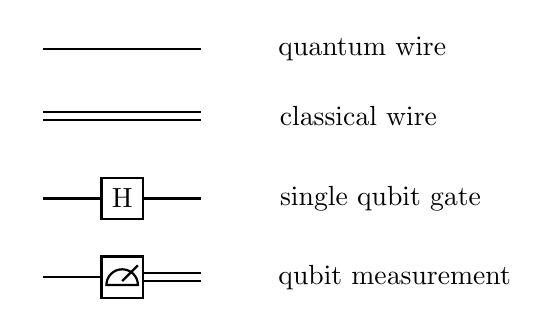
\begin{tikzpicture}[thick]
			
			\tikzstyle{operator} = [draw,fill=white,minimum size=1.5em] 
			
			%\draw (3,3) -- (3,0) ;
			
			\draw (0,3) -- (2,3) ;
			\node at (4.05,3) {quantum wire};
			
			\draw (0,2.1) -- (2,2.1) ;
			\draw (0,2.2) -- (2,2.2) ;
			\node at (4,2.15) {classical wire};
			
			\draw (0,1.1) -- (2,1.1) ;
			\node[operator] (op11) at (1,1.1) {H};
			\node at (4.28,1.1) {single qubit gate};
			
			\draw (0,0.1) -- (1,0.1) ;
			
			\draw (1,0.15) -- (2,0.15) ;
			\draw (1,0.05) -- (2,0.05) ;
			% Define coordinates
			\def\Radius{0.2}
			\path
			(-\Radius, 0) coordinate (A)
			-- coordinate (M)
			(\Radius, 0) coordinate (B)
			(M) +(60:\Radius) coordinate (C)
			+(120:\Radius) coordinate (D)
			;
			
			\node[operator] (op11) at (1,0.1) {};
			\node at (4.46,0.1) {qubit measurement};
			
			% Draw semicircle
			\draw[operator]
			(1.2,0) arc(0:180:\Radius) -- cycle ;
			% Annotations
			
			\draw (1,0.05) -- (1.2,0.25);
			
		\end{tikzpicture}
	\end{figure}	
	
	\subsection{Controlled Gates and Phase Kickback}
	
	\textbf{section not complete}
	
	\begin{enumerate}
		\item We will describe the use of control gates.
		\item We will describe the emergence of phase kickback with the use of hadamard gates discussed in the previous section. This will be important to know going into the next section.
	\end{enumerate}
	
	\section{Quantum Phase Estimation}
	
	The phase estimation algorithm initially proposed by Alexey Kitaev \cite{kitaev1995quantum} plays an important role as a subroutine for the more widely known factoring algorithm by Peter Shor \cite{Shor}. We first must briefly discuss the Quantum Fourier Transform (QFT) as it is key to understanding phase estimation \cite{nielsen00}. Given a computational basis state $|x\rangle$, applying the QFT ($F_N$) results in:
	
	$$ F_N |x \rangle = \frac{1}{\sqrt{N}} \sum_{k=0}^{N-1} e^{2\pi i x k N^{-1}} |k\rangle $$
	
	Let's represent this in binary notation and decompose it into a tensor product. We can represent $|x\rangle$ as a string of bits, and the QFT as a tensor product of single qubit basis states:
	
	$$|x\rangle = |x_1x_2 ... x_n\rangle =  |x_1\rangle \otimes |x_2\rangle \otimes ... \otimes |x_n\rangle$$
	
	\begin{eqnarray}
		F_N |x \rangle = \frac{1}{\sqrt{2^n}} \bigotimes_{j=1}^n (|0\rangle +  e^{2\pi i x 2^{-j}} |1\rangle)
	\end{eqnarray}
	
	$$= \frac{1}{\sqrt{2^n}} ((|0\rangle + \omega_1|1\rangle)  \otimes(|0\rangle + \omega_2|1\rangle)\otimes ... \otimes(|0\rangle + \omega_n|1\rangle))$$
	
	
	\begin{eqnarray*}
		\omega_1 &=& e^{2\pi i x 2^{-1}} =  e^{2\pi i (0.x_n)}\\
		\omega_2 &=& e^{2\pi i x 2^{-2}} =  e^{2\pi i (0.x_{n-1}x_n)}\\
		...\\
		\omega_n &=& e^{2\pi i x 2^{-n}} =  e^{2\pi i (0.x_1...x_n)}
	\end{eqnarray*}
	
	
	An important characteristic of the $w_j$ is the bit shift occurring in the exponent. If we look at $w_1$, the exponent has a factor $x 2^{-1}$, which is equivalent to one right bit shift: $x_1...x_{n-1}.x_n$. Integer multiples of the exponent would imply full rotations returning to the same point thus we can ignore all the values on the left of the decimal and what remains is $0.x_n$. 
	
	
	
	Let's discuss the phase estimation problem. Given an eigenstate $|\lambda \rangle$ of a unitary operator $U$, we want to calculate a good approximation  for $\phi \in [0,1)$ satisfying:
	
	\begin{equation}
		U |\lambda \rangle = e^{2\pi i \phi} |\lambda \rangle
	\end{equation}
	
	The phase estimation algorithm uses two registers of qubits. The first one will be a set of $n$ control qubits that determine the precision of our approximation. The second register will be a set of $m$ qubits initialized to an eigenstate $|\lambda\rangle$.
	
	
	\begin{figure}[!h]
		\centering
		\includegraphics[trim={1cm 12cm 11cm 0},clip, width=0.8 \linewidth]{"graphics/phase_circ"}
		\caption{A quantum circuit representation of the phase estimation algorithm. Given, $ U |\lambda \rangle = e^{2\pi i \phi} |\lambda \rangle $, this algorithm allows us to generate an  approximation for $\phi \in [0,1)$ . The circuit consists of two registers of qubits, the first $n$-qubits are initialized to $|0\rangle$ and contribute to the precision of the $\phi$ value obtained. The second register of $m$-qubits is initialized to the eigenstate of $U$.  The Hadamard gates, $H$, are used to create a uniform superposition in the first register. The control gates based on $U$ are responsible for encoding phase to the qubits in the first register. Finally, a $QFT^\dagger$ is performed on the first register to extract the encoded phase. Each subsequent qubit in the first register would require double the control gates. Thus, with a large $n$ we obtain a more precise value for $\phi$, but also exponentially increase our computation time.}
		\label{fig:phasrcircuit}
	\end{figure}
	
	
	Let's walk through the quantum circuit in FIG. \ref{fig:phasrcircuit}, to understand the inner workings of this algorithm.	 Our initialized state is $|0^{\otimes n} \lambda\rangle$. From here we perform the same operation we find in equation 1, where all the qubits in the first register are set to a uniform superposition on all states $2^n$. The next portion of the algorithm involves applying controlled gates based on the unitary operator $U$. The function of these $CU$ gates is to apply the operator $U$ on $|\lambda\rangle$ if the control qubit is in the state $|1\rangle$. We can have a look at the effect on the n\textsuperscript{th} qubit, after it has been prepared in a superposition by the Hadamard gate:
	
	$$ \frac{1}{\sqrt{2}}(|0\rangle + |1\rangle) \otimes |\lambda\rangle = |0 \lambda \rangle + |1 \lambda\rangle$$
	
	Applying $CU$ and factoring out the eigenstate:
	
	\begin{eqnarray*}
		CU \frac{1}{\sqrt{2}}(|0 \lambda \rangle + |1 \lambda\rangle) &=&  \frac{1}{\sqrt{2}}(CU|0 \lambda \rangle + CU|1 \lambda\rangle )\\
		&=& \frac{1}{\sqrt{2}}(|0 \lambda \rangle + e^{2\pi i \phi}|1 \lambda\rangle)\\
		&=&\frac{1}{\sqrt{2}}( |0 \rangle + e^{2\pi i \phi}|1 \rangle)\otimes |\lambda\rangle
	\end{eqnarray*}
	
	We can see the eigenstate after the $CU$ operation is left unchanged. the phase has been encoded into the control qubit instead, a result is due to the phase kickback. Thus, we can reuse our eigenstate for the next qubit. Consecutive qubits have double the amount of $CU$ operators as the previous, thus squaring the eigenvalue each time:
	
	\begin{eqnarray*}
		\text{qubit\textsubscript{n-1}} &:&   |0 \rangle + e^{2\pi i \phi 2}|1 \rangle \\
		...\\
		\text{qubit\textsubscript{1}} &:&   |0 \rangle + e^{2\pi i \phi 2^n}|1 \rangle
	\end{eqnarray*}
	
	We know that the value of $\phi < 1$. We can represent this in binary notation in the form $0.\phi_1\phi_2...\phi_n$:
	
	$$\phi = \sum_{j=1}^n \phi_j 2^{-j}$$
	
	If we have another look at the control qubits using binary notation for $\phi$ instead, we can see the result of the multiple $CU$ operations simply results in right bit shifts:
	
	
	\begin{eqnarray*}
		\text{qubit\textsubscript{n}} &:&   |0 \rangle +e^{2\pi i (0.\phi_1\phi_2...\phi_n)}|1 \rangle  \\
		\text{qubit\textsubscript{n-1}} &:&   |0 \rangle + e^{2\pi i (0.\phi_2...\phi_n)}|1 \rangle \\
		...\\
		\text{qubit\textsubscript{1}} &:&   |0 \rangle + e^{2\pi i (0.\phi_n)}|1 \rangle
	\end{eqnarray*}
	
	If we look at the form of first register after all the $CU$ operations in the state $|\alpha\rangle$, it will resemble the result of performing the QFT we saw in equation 5. Where our $\omega_j$ are:
	
	\begin{eqnarray*}
		\omega_1 &=& e^{2\pi i x 2^{-1}} =  e^{2\pi i (0.\phi_n)}\\
		\omega_2 &=& e^{2\pi i x 2^{-2}} =  e^{2\pi i (0.\phi_{n-1}\phi_n)}\\
		...\\
		\omega_n &=& e^{2\pi i x 2^{-n}} =  e^{2\pi i (0.\phi_1...\phi_n)}
	\end{eqnarray*}
	
	simply performing the inverse QFT will give us $|\phi\rangle =  |\phi_1\phi_2 ... \phi_n\rangle$.  We can immediately see the approximation is limited by the number of qubits in the first register. A simple strategy would be to increase the number of qubits; however this would also increase computational cost as we double our use of $CU$ gates for each additional qubit.
	
	
	
	
	
	%A simple example of minimizing the bottleneck travelling salesman problem (maybe with images):
	%an example of storing phases and using phase estimation
	%grover's search explanation
	\chapter{Algorithm for the Constraint Problem}
	
The constrained version of the BTSP asks whether there exists a Hamiltonian cycle in which the weight of every edge is less than a specified threshold $\alpha$. In such a cycle, if we denote the weight of any edge as $\gamma_i$, then it must satisfy the condition:
	 
	 $$\gamma_i < \alpha$$
	
	
	We will construct the algorithm in the following steps:
	\begin{enumerate}
		\item Normalize edge weights so no single hamiltonian cycle is greater than or equal to 1. This is to ensure we can appropriately use the phase estimation algorithm.\\
		\item Construct a unitary operator that holds information regarding the hamiltonian cyles as phases in the diagonal. The approach will follow inline with what was found  the paper: \cite{srinivasan2018efficient} \\
		\item Set all edgeweights $> \alpha$ to zero and construct a secondary unitary operator similiar to step 2.\\
		\item Create controlled gates using the unitary operators constructed in Step 2 and 3.\\
		\item Identify all the eigenstates of the unitary operators that map to the phases associated with the hamiltonian cycles.\\
		\item Perform phase estimation twice with an eigenstate using the control gates to evaluate the hamiltonian cycle before and after the edgeweights $> \alpha$ are set to zero.\\
		\item Compare the two phases achieved. If they are equal, the corresponding hamiltonian cycle is a solution that satisfies the constraint.\\
		
	\end{enumerate}
		
	\section{Normalize Edge Weights}
	
	A hamiltonian cycle of a complete graph with $N$ nodes requires $N$ edge-weights to complete the cycle. A single graph consists a total of $N(N-1)$ edgeweights in a directed graph. we can choose the largest $N$ and use these to normalize the edge weights. Let $w$ describe our edge-weights and will be a list of $m = N(N-1)$ elements:
	
	$$w = \{w_1, w_2, \ldots, w_m\}$$ 
	
	Sort $w$ in descending order to obtain:
	
	\begin{equation}\label{sorted-weights}
	w' = \{w'_1, w'_2, \ldots, w'_m\}
	\end{equation}
	
	Where: $w'_1 \geq w'_2 \geq \ldots \geq w'_m$
	
	\vspace{0.5cm}
	
The sum $S$ of the largest $N$ items in $w$ can be described as:

\begin{equation}\label{sum-S}
S = \sum_{i=1}^{N} w'_i
\end{equation}

  We can now perform the normalization. Let $\tilde{w}$ describe our normalized edge-weights:
  
 \begin{equation}\label{normalization}
  	\tilde{w} = (S + \epsilon)^{-1}w
\end{equation}

		Where: $\epsilon>0$.  The purpose of $\epsilon$ is to make sure if any normalized hamiltonian cycle is exactly equal to $ S$ then we do not have a zero phase.
	
	
	\section{Unitary Operator and Eigenstates associated with the Hamiltonian Cycles}
	
	 We start by constructing diagonal matrices $U_j$, one for each node in a complete graph and describe the matrix elements:
	
	\begin{equation}\label{Uj-elements}
	\left[U_j \right]_{kk} = e^{2\pi i\gamma_{jk} (1 - \delta_{jk})}
	\end{equation}
	
	Where:	$ 1 \leq j, k \leq N$
	$N$ denotes the total number of nodes.
	$\gamma_{jk}$ represents the edgeweight connecting node $j\rightarrow k$
	
	\vspace{0.5cm}
	
	Then we construct $U$, a tensor product of all the diagonal matrices:
	\begin{equation}\label{U-tensor}
	 U = \bigotimes_j^N U_j
	 \end{equation}
	
	
	$U$ will be a $N^N \times N^N$ matrix with only the diagonal elements populated. Because the diagonal elements will entirely consist of phases $\left[U \right]_{kk} = e^{i\alpha_{kk}} $. We can confirm the unitary operator condition is satisfied: $U^\dagger U = \mathds{1}$. 
	
	
	Given $U$'s diagonal nature, its eigenstates align with the basis vectors. Our focus is on specific eigenstates corresponding to the Hamiltonian cycles, determined by the phases. To comprehend how the diagonal elements of $U$ derive from the individual $U_j$ matrices, we visualize the tensor product construction. Notably, the product populates the diagonal elements of $U$ allowing a simplification where we consider these elements directly:
	
	\begin{flalign*}
	[U]_{0} & = [U_1]_{0}\cdot [U_2] _{0}\cdot \ldots  \cdot [U_{N-2}]_{0} \cdot [U_{N-1}]_{0}\cdot [U_N]_{0} \\
	[U]_{1}  & = [U_1]_{0}\cdot [U_2] _{0}\cdot \ldots \cdot [U_{N-2}]_{0}\cdot [U_{N-1}]_{0}\cdot [U_N]_{1}\\
	&  \vdots\\
	[U]_{N-1} &= [U_1]_{0}\cdot [U_2] _{0}\cdot \ldots\cdot [U_{N-2}]_{0} \cdot [U_{N-1}]_{0}\cdot [U_N]_{N-1}\\
	[U]_{N} &= [U_1]_{0}\cdot [U_2] _{0}\cdot \ldots \cdot [U_{N-2}]_{0} \cdot [U_{N-1}]_{1}\cdot [U_N]_{0}\\
	& \vdots\\
	[U]_{2N - 1} & = [U_1]_{0}\cdot [U_2] _{0}\cdot \ldots \cdot [U_{N-2}]_{0} \cdot [U_{N-1}]_{1}\cdot [U_N]_{N-1}\\
	[U]_{2N} &= [U_1]_{0}\cdot [U_2] _{0}\cdot \ldots \cdot [U_{N-2}]_{0} \cdot [U_{N-1}]_{2}\cdot [U_N]_{0}\\
	& \vdots\\
	[U]_{N^2 - 1 } & = [U_1]_{0}\cdot [U_2] _{0}\cdot \ldots \cdot [U_{N-2}]_{0} \cdot [U_{0}]_{N-1}\cdot [U_N]_{N-1}\\
	[U]_{N^2} &= [U_1]_{0}\cdot [U_2] _{0}\cdot \ldots \cdot [U_{N-2}]_{1} \cdot [U_{N-1}]_{0}\cdot [U_N]_{0}\\
	& \vdots\\
	[U]_{N^2 + N - 1} & = [U_1]_{0}\cdot [U_2] _{0}\cdot \ldots \cdot [U_{N-2}]_{1} \cdot [U_{N-1}]_{0}\cdot [U_N]_{N-1}\\
	[U]_{N^2 + N } &= [U_1]_{0}\cdot [U_2] _{0}\cdot \ldots \cdot [U_{N-2}]_{1} \cdot [U_{N-1}]_{1}\cdot [U_N]_{0}\\
	&  \vdots\\
	[U]_{N^3- 1} & = [U_1]_{0}\cdot [U_2] _{0}\cdot \ldots \cdot [U_{N-2}]_{N-1} \cdot [U_{N-1}]_{N-1}\cdot [U_N]_{N-1}
	\end{flalign*}
	\vspace{0.5cm}
	This pattern indicates:
	\begin{equation}\label{U-matrix-eq}
	[U]_{k} = [U_1]_{\alpha_{N-1}}\cdot [U_2] _{\alpha_{N-2}}\cdot \ldots \cdot [U_{N-2}]_{\alpha_2} \cdot [U_{2}]_{\alpha_{1}}\cdot [U_N]_{\alpha_{0}}
	\end{equation}
	
	With: $$\alpha_i = \left(k//\left(N^{i}\right)\right) \% N$$
	
	\vspace{0.5cm}
	
	Where:
	
	$//$ denotes integer division
	
	$\%$ is the modulus operation
	
	\vspace{0.5cm}
	
 	We can see the pattern follows base-$N$ counting where $N$ is the total number of nodes. Simply converting $k$ into base-$N$, will give us the indices of our original diagonal matrices. To locate the relevent eigenstates, we start by identifying the elements in $U_j$ associated  with a hamiltonian cycle, retrieve their respective indices, convert this string of indices from Base-$N$ to $k$.  and we would have identified our eigenstate $|k\rangle$. 
	
	\subsection{The Four City Graph}
	
	\begin{center}	
	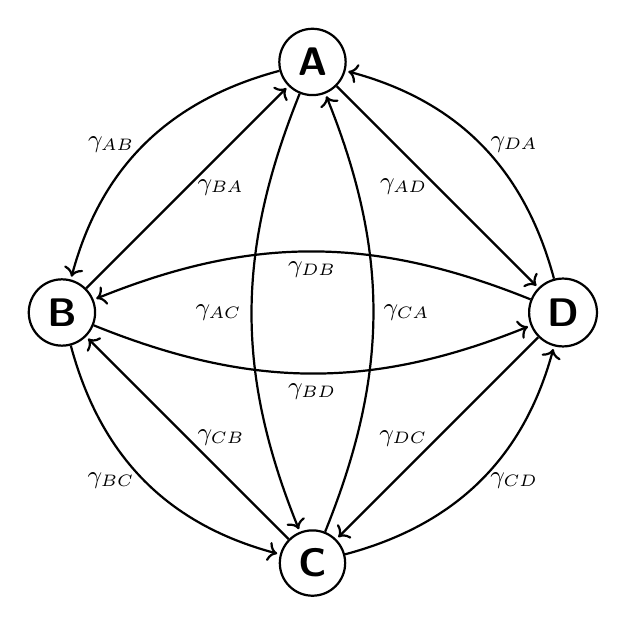
\begin{tikzpicture}[->,shorten >=1pt,auto,node distance=4.5cm, thick,main node/.style={circle,draw,font=\sffamily\Large\bfseries}]
		
		\node[main node] (1) {A};
		\node[main node] (2) [below left of=1] {B};
		\node[main node] (3) [below right of=2] {C};
		\node[main node] (4) [below right of=1] {D};
		
		\path[every node/.style={font=\sffamily\small}]
		(1) edge node [left] {$\gamma_{AD}$} (4)
		edge [bend right] node[left] {$\gamma_{AB}$} (2)
		edge[bend right=22] node[left] {$\gamma_{AC}$} (3)
		%edge [loop above] node {0.1} (1)
		(2) edge node [right] {$\gamma_{BA}$} (1)
		edge[bend right=22] node[below] {$\gamma_{BD}$} (4)
		%edge [loop left] node {0.4} (2)
		edge [bend right] node[left] {$\gamma_{BC}$} (3)
		(3) edge node [right] {$\gamma_{CB}$} (2)
		edge [bend right] node[right] {$\gamma_{CD}$} (4)
		edge[bend right=22] node[right] {$\gamma_{CA}$} (1)
		(4) edge node [left] {$\gamma_{DC}$} (3)
		%edge [loop right] node {0.6} (4)
		edge[bend right=22] node {$\gamma_{DB}$} (2)
		edge [bend right] node[right] {$\gamma_{DA}$} (1);
	\end{tikzpicture}
	
	\end{center}
	
	
	For the 4 city problem we will start with four matrices to represent the $12$ edgeweights from each node. Using \ref{Uj-elements}, Where:	$ j, k \in \{A,B,C,D\}$.  we can construct matrix $A$:

	$$
	A = \begin{bmatrix}
		1 & 0 & 0 & 0 \\
		0 & e^{i2\pi\gamma_{AB}} & 0 & 0 \\
		0 & 0 & e^{i2\pi\gamma_{AC}} & 0 \\
		0 & 0 & 0 & e^{i2\pi\gamma_{AD}} \\
	\end{bmatrix}
	$$
	
	Since we only populate the diagonal elements, we can ignore the other elements of the matrix. Let $ a = \mathrm{diag}(A)$, and lets construct the other diagonals:
	
	\begin{align*}	
		a & = \begin{bmatrix}
			1 \\
			e^{i2\pi\gamma_{AB}} \\
			e^{i2\pi\gamma_{AC}} \\
			e^{i2\pi\gamma_{AD}} \\
		\end{bmatrix} 
		b  = \begin{bmatrix}
			e^{i2\pi\gamma_{BA}} \\
			1 \\
			e^{i2\pi\gamma_{BC}} \\
			e^{i2\pi\gamma_{BD}} \\
		\end{bmatrix}
		c  = \begin{bmatrix}
			e^{i2\pi\gamma_{CA}} \\
			e^{i2\pi\gamma_{CB}} \\
			1 \\
			e^{i2\pi\gamma_{CD}} \\
		\end{bmatrix} 
		d = \begin{bmatrix}
			e^{i2\pi\gamma_{DA}} \\
			e^{i2\pi\gamma_{DB}} \\
			e^{i2\pi\gamma_{DC}} \\
			1 \\
		\end{bmatrix} 						 			
	\end{align*}
	
	
	We then construct the tensor product with equation \ref{U-tensor}:
	
	\begin{equation}\label{4-city-matrix-tensor}
	 U = A \otimes B \otimes C \otimes D
	\end{equation}
	
	The convience of dealing with only the diagonals we can similiarly state $ u = \mathrm{diag}(U)$, thus:
	
	$$ u = a \otimes b \otimes c \otimes d$$
	
	
	Refering to equation \ref{U-matrix-eq} regarding the matrix elements for U,  the diagonal elements for the 4-city problem will reduce to:
	
	\begin{equation}\label{4-city-tensor}
		u_{k} = a_{\alpha_{3}}\cdot b _{\alpha_{2}} \cdot c_{\alpha_1} \cdot d_{\alpha_{0}}
	\end{equation}
	
	With: $$\alpha_i = \left(k//\left(4^{i}\right)\right) \% 4$$
	
	
	\vspace{0.5cm}
	
	lets walk through identifying the eigenstate of one hamiltonian cycle. Lets say the cycle we choose is the following:
	
	\begin{equation}\label{one-ham-cycle-4-city}
		A \rightarrow D \rightarrow B \rightarrow C \rightarrow A
	\end{equation}
	from here we can identify the edgeweights we care about are:
	
	\begin{equation*}
		\gamma_{AD} + \gamma_{DB} + \gamma_{BC} + \gamma_{CA}
	\end{equation*}
	
	Thus the phase we would like to estimate would be given by the following element product:
	
	\begin{equation*}
		\Large{a_{3} \cdot d_{1} \cdot b_{2} \cdot c_{0} = e^{i2\pi (\gamma_{AD} + \gamma_{DB} + \gamma_{BC} + \gamma_{CA})}}
	\end{equation*}
	
	
	To correctly identify the eigenstate, we need to rearrange the product to match the form of equation \ref{4-city-tensor}:
	
	\begin{equation*}
		\Large{a_{3} \cdot d_{1} \cdot b_{2} \cdot c_{0} = \Large{a_{3}} \cdot b_{2} \cdot c_{0}  \cdot d_{1}}
	\end{equation*}
	
	From here we simply read out the indices and based on our discussion under equation \ref{U-matrix-eq} , we can infer we are working in base 4. Thus we simply need to convert to base 10 to understand the exact column number and to base 2 to be used as the initialized eigenstate.
	
	\begin{equation*}
		\text{base } 4 = 3201 \leftrightarrow \text{base } 10 = 225 \leftrightarrow  \text{base } 2 = 11100001
	\end{equation*}
	
	Thus our eigenstate for \ref{one-ham-cycle-4-city} will be  $|225\rangle$ or $|11100001\rangle$. We can perform an identical process for all the hamiltonian cycles to find their corresponding eigenstates. These are all listed in table \ref{table:ham-cycle-details-4-city} and and \ref{table:4-city-conversions}
	
	
	\begin{table}[h]
		\centering
		\begin{tabular}{|c|c|c|}
			\hline
			\textbf{Hamiltonian Cycle} & \textbf{Edge Weights Sum} & \textbf{Diagonal Elements Product} \\
			\hline
			$A \rightarrow B \rightarrow C \rightarrow D \rightarrow A$ & $\gamma_{AB} + \gamma_{BC} + \gamma_{CD} + \gamma_{DA}$ & $a_{1} \cdot b_{2} \cdot c_{3} \cdot d_{0}$ \\
			$A \rightarrow B \rightarrow D \rightarrow C \rightarrow A$ & $\gamma_{AB} + \gamma_{BD} + \gamma_{DC} + \gamma_{CA}$ & $a_{1} \cdot b_{3} \cdot d_{2} \cdot c_{0}$ \\
			$A \rightarrow C \rightarrow B \rightarrow D \rightarrow A$ & $\gamma_{AC} + \gamma_{CB} + \gamma_{BD} + \gamma_{DA}$ & $a_{2} \cdot c_{1} \cdot b_{3} \cdot d_{0}$ \\
			$A \rightarrow C \rightarrow D \rightarrow B \rightarrow A$ & $\gamma_{AC} + \gamma_{CD} + \gamma_{DB} + \gamma_{BA}$ & $a_{2} \cdot c_{3} \cdot d_{1} \cdot b_{0}$ \\
			$A \rightarrow D \rightarrow B \rightarrow C \rightarrow A$ & $\gamma_{AD} + \gamma_{DB} + \gamma_{BC} + \gamma_{CA}$ & $a_{3} \cdot d_{1} \cdot b_{2} \cdot c_{0}$ \\
			$A \rightarrow D \rightarrow C \rightarrow B \rightarrow A$ & $\gamma_{AD} + \gamma_{DC} + \gamma_{CB} + \gamma_{BA}$ & $a_{3} \cdot d_{2} \cdot c_{1} \cdot b_{0}$ \\
			\hline
			\end{tabular}
					\caption{Hamiltonian cycles of the directed 4-city graph with their edgeweight summation and expected diagonal element products (\ref{4-city-tensor}).}
			\label{table:ham-cycle-details-4-city}
	\end{table}
	\begin{table}[h]
		\centering
		\begin{tabular}{|c|c|c|}	
			
			\hline
			\textbf{Rearranged Indices (Base 4)} & \textbf{Base 10} & \textbf{Base 2} \\
			\hline
			1230 & 108 & 01101100 \\
			1302 & 114 & 01110010 \\
			2310 & 180 & 10110100 \\
			2031 & 141 & 10001101 \\
			3201 & 225 & 11100001 \\
			3012 & 198 & 11000110 \\
			\hline
		\end{tabular}
		\caption{Eigenstates of matrix $U$ (\ref{4-city-matrix-tensor}), containing the normalized hamiltonian cycle edge weight sum of the directed 4-city graph.}
		\label{table:4-city-conversions}
	\end{table}
	
	\subsection{The Five City Graph}
	
	
	
		\begin{center}	
		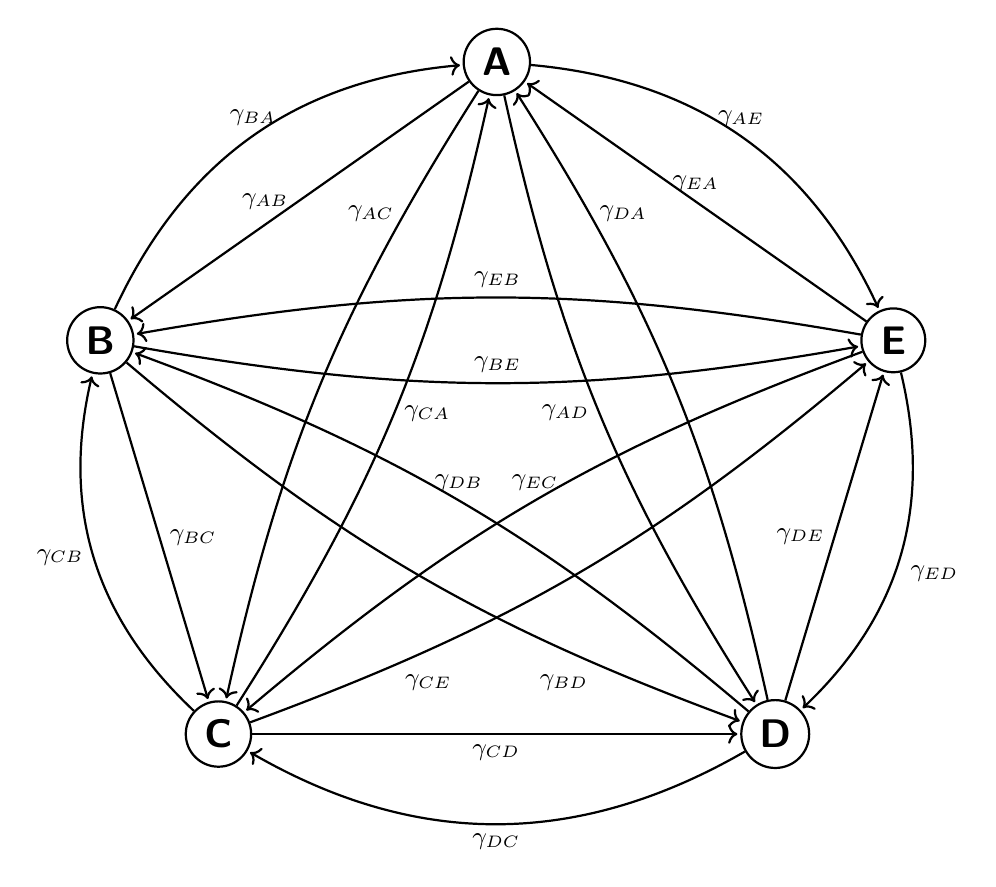
\begin{tikzpicture}[->,shorten >=1pt,auto,node distance=5cm, thick,main node/.style={circle,draw,font=\sffamily\Large\bfseries}]
			
			\node[main node] (1) {A};
			\node[main node] (2) [below left of=1, xshift = -1.5cm] {B};
			\node[main node] (3) [below of=2, xshift= 1.5cm] {C};
			\node[main node] (5) [below right of=1, xshift = 1.5cm] {E};
			\node[main node] (4) [below of=5, xshift= -1.5cm] {D};
			
			\path[every node/.style={font=\sffamily\small}]
			(1) edge [bend right=10] node [left] {$\gamma_{AD}$} (4)
			edge node[left] {$\gamma_{AB}$} (2)
			edge [bend right=10] node[left, pos = 0.2] {$\gamma_{AC}$} (3)
			edge[bend left] node[above] {$\gamma_{AE}$} (5)

			(2) edge[bend left] node [above] {$\gamma_{BA}$} (1)
			edge [bend right=10]  node[below left , pos = 0.8] {$\gamma_{BD}$} (4)
			edge node[right] {$\gamma_{BC}$} (3)
			edge [bend right=10] node[above] {$\gamma_{BE}$} (5)
			
			(3) edge[bend left] node [left] {$\gamma_{CB}$} (2)
			edge node[below] {$\gamma_{CD}$} (4)
			edge [bend right=10] node[right] {$\gamma_{CA}$} (1)
			edge [bend right=10] node[below right , pos = 0.2] {$\gamma_{CE}$} (5)
			
			(4) edge[bend left] node[below] {$\gamma_{DC}$} (3)
			edge [bend right=10] node[above] {$\gamma_{DB}$} (2)
			edge [bend right=10] node[right, pos = 0.8] {$\gamma_{DA}$} (1)
			edge node[left] {$\gamma_{DE}$} (5)
			
			(5) edge node [above] {$\gamma_{EA}$} (1)
			edge [bend right=10]  node[above] {$\gamma_{EB}$} (2)
			edge [bend right=10] node[above] {$\gamma_{EC}$} (3)
			edge[bend left] node {$\gamma_{ED}$} (4);

		\end{tikzpicture}
		
	\end{center}
	
	
	We construct our matrix U with the tensor product as in equation \ref{U-tensor}.
	
	\begin{equation}\label{5-city-matrix-tensor}
		U = A \otimes B \otimes C \otimes D \otimes E
	\end{equation}
	
	 Similiar to the four-city graph we only populate the diagonal elements, Let $ a = \mathrm{diag}(A)$, and let us construct the other diagonals:
	
	\begin{align*}	
		a & = \begin{bmatrix}
			1 \\
			e^{i2\pi\gamma_{AB}} \\
			e^{i2\pi\gamma_{AC}} \\
			e^{i2\pi\gamma_{AD}} \\
			e^{i2\pi\gamma_{AE}} \\
		\end{bmatrix} 
		b  = \begin{bmatrix}
			e^{i2\pi\gamma_{BA}} \\
			1 \\
			e^{i2\pi\gamma_{BC}} \\
			e^{i2\pi\gamma_{BD}} \\
			e^{i2\pi\gamma_{BE}} \\
		\end{bmatrix}
		c  = \begin{bmatrix}
			e^{i2\pi\gamma_{CA}} \\
			e^{i2\pi\gamma_{CB}} \\
			1 \\
			e^{i2\pi\gamma_{CD}} \\
			e^{i2\pi\gamma_{CE}} \\
		\end{bmatrix} 
		d = \begin{bmatrix}
			e^{i2\pi\gamma_{DA}} \\
			e^{i2\pi\gamma_{DB}} \\
			e^{i2\pi\gamma_{DC}} \\
			1 \\
			e^{i2\pi\gamma_{DE}} \\
		\end{bmatrix}  
		e = \begin{bmatrix}
			e^{i2\pi\gamma_{EA}} \\
			e^{i2\pi\gamma_{EB}} \\
			e^{i2\pi\gamma_{EC}} \\
			e^{i2\pi\gamma_{ED}} \\
			1 \\
		\end{bmatrix}		 			
	\end{align*}
	

	
	We can state $ u = \mathrm{diag}(U)$, thus:
	
	$$ u = a \otimes b \otimes c \otimes d \otimes e$$
	
	
	Refering to equation \ref{U-matrix-eq} regarding the matrix elements for U,  the diagonal elements for the 5-city problem will reduce to:
	
	\begin{equation}\label{5-city-tensor}
		u_{k} = a_{\alpha_{4}}\cdot b _{\alpha_{3}} \cdot c_{\alpha_2} \cdot d_{\alpha_{1}}\cdot e_{\alpha_{0}}
	\end{equation}
	
	With: $$\alpha_i = \left(k//\left(5^{i}\right)\right) \% 5$$
	
	
	\vspace{0.5cm}
	
	Let us walk through identifying the eigenstate of one hamiltonian cycle:
	
	\begin{equation}\label{one-ham-cycle-4-city}
		A \rightarrow E \rightarrow D \rightarrow C \rightarrow B \rightarrow A
	\end{equation}
	
	from here we can identify the edgeweights we care about are:
	
	\begin{equation*}
		\gamma_{AE} + \gamma_{ED} + \gamma_{DC} + \gamma_{CB} + \gamma_{BA}
	\end{equation*}
	
	Thus the phase we would like to estimate would be given by the following element product:
	
	\begin{equation*}
		\Large{a_{4} \cdot e_{3} \cdot d_{2} \cdot c_{1} \cdot b_{0} = e^{i2\pi (\gamma_{AE} + \gamma_{ED} + \gamma_{DC} + \gamma_{CB} + \gamma_{BA})}}
	\end{equation*}
	
	
	To correctly identify the eigenstate, we need to rearrange the product to match the form of equation \ref{5-city-tensor}:
	
	\begin{equation*}
		\Large{a_{4} \cdot e_{3} \cdot d_{2} \cdot c_{1} \cdot b_{0}= a_{4} \cdot b_{0}  \cdot c_{1}\cdot d_{2} \cdot e_{3}}
	\end{equation*}
	
	From here we simply read out the indices and based on our discussion under equation \ref{U-matrix-eq} , we can infer we are working in base 4. Thus we simply need to convert to base 10 to understand the exact column number and to base 2 to be used as the initialized eigenstate.
	
	\begin{equation*}
		\text{base } 5 = 40123 \leftrightarrow \text{base } 10 = 2538 \leftrightarrow  \text{base } 2 = 100111101010
	\end{equation*}
	
	Thus our eigenstate for \ref{one-ham-cycle-4-city} will be  $|2538\rangle$ or $|100111101010\rangle$. We can perform an identical process for all the hamiltonian cycles to find their corresponding eigenstates. These are all listed in table \ref{table:ham-cycle-details-5-city} and \ref{table:5-city-conversions}
	
	
	
	
	\begin{table}[h]
		\centering
		\begin{tabular}{|c|c|c|}
			\hline
			\textbf{Hamiltonian Cycle} & \textbf{Edge Weights Sum} & \textbf{Matrix Elements Product} \\
			\hline
$A \rightarrow B \rightarrow C \rightarrow D \rightarrow E \rightarrow A$ & $ \gamma_{AB} + \gamma_{BC} + \gamma_{CD} + \gamma_{DE} + \gamma_{EA}$ & $a_1  \cdot b_2 \cdot c_3 \cdot d_4 \cdot e_0$ \\
$A \rightarrow B \rightarrow C \rightarrow E \rightarrow D \rightarrow A$ & $ \gamma_{AB} + \gamma_{BC} + \gamma_{CE} + \gamma_{ED} + \gamma_{DA}$ & $a_1  \cdot b_2 \cdot c_4 \cdot e_3 \cdot d_0$ \\
$A \rightarrow B \rightarrow D \rightarrow C \rightarrow E \rightarrow A$ & $ \gamma_{AB} + \gamma_{BD} + \gamma_{DC} + \gamma_{CE} + \gamma_{EA}$ & $a_1  \cdot b_3 \cdot d_2 \cdot c_4 \cdot e_0$ \\
$A \rightarrow B \rightarrow D \rightarrow E \rightarrow C \rightarrow A$ & $ \gamma_{AB} + \gamma_{BD} + \gamma_{DE} + \gamma_{EC} + \gamma_{CA}$ & $a_1  \cdot b_3 \cdot d_4 \cdot e_2 \cdot c_0$ \\
$A \rightarrow B \rightarrow E \rightarrow C \rightarrow D \rightarrow A$ & $ \gamma_{AB} + \gamma_{BE} + \gamma_{EC} + \gamma_{CD} + \gamma_{DA}$ & $a_1  \cdot b_4 \cdot e_2 \cdot c_3 \cdot d_0$ \\
$A \rightarrow B \rightarrow E \rightarrow D \rightarrow C \rightarrow A$ & $ \gamma_{AB} + \gamma_{BE} + \gamma_{ED} + \gamma_{DC} + \gamma_{CA}$ & $a_1  \cdot b_4 \cdot e_3 \cdot d_2 \cdot c_0$ \\
$A \rightarrow C \rightarrow B \rightarrow D \rightarrow E \rightarrow A$ & $ \gamma_{AC} + \gamma_{CB} + \gamma_{BD} + \gamma_{DE} + \gamma_{EA}$ & $a_2  \cdot c_1 \cdot b_3 \cdot d_4 \cdot e_0$ \\
$A \rightarrow C \rightarrow B \rightarrow E \rightarrow D \rightarrow A$ & $ \gamma_{AC} + \gamma_{CB} + \gamma_{BE} + \gamma_{ED} + \gamma_{DA}$ & $a_2  \cdot c_1 \cdot b_4 \cdot e_3 \cdot d_0$ \\
$A \rightarrow C \rightarrow D \rightarrow B \rightarrow E \rightarrow A$ & $ \gamma_{AC} + \gamma_{CD} + \gamma_{DB} + \gamma_{BE} + \gamma_{EA}$ & $a_2  \cdot c_3 \cdot d_1 \cdot b_4 \cdot e_0$ \\
$A \rightarrow C \rightarrow D \rightarrow E \rightarrow B \rightarrow A$ & $ \gamma_{AC} + \gamma_{CD} + \gamma_{DE} + \gamma_{EB} + \gamma_{BA}$ & $a_2  \cdot c_3 \cdot d_4 \cdot e_1 \cdot b_0$ \\
$A \rightarrow C \rightarrow E \rightarrow B \rightarrow D \rightarrow A$ & $ \gamma_{AC} + \gamma_{CE} + \gamma_{EB} + \gamma_{BD} + \gamma_{DA}$ & $a_2  \cdot c_4 \cdot e_1 \cdot b_3 \cdot d_0$ \\
$A \rightarrow C \rightarrow E \rightarrow D \rightarrow B \rightarrow A$ & $ \gamma_{AC} + \gamma_{CE} + \gamma_{ED} + \gamma_{DB} + \gamma_{BA}$ & $a_2  \cdot c_4 \cdot e_3 \cdot d_1 \cdot b_0$ \\
$A \rightarrow D \rightarrow B \rightarrow C \rightarrow E \rightarrow A$ & $ \gamma_{AD} + \gamma_{DB} + \gamma_{BC} + \gamma_{CE} + \gamma_{EA}$ & $a_3  \cdot d_1 \cdot b_2 \cdot c_4 \cdot e_0$ \\
$A \rightarrow D \rightarrow B \rightarrow E \rightarrow C \rightarrow A$ & $ \gamma_{AD} + \gamma_{DB} + \gamma_{BE} + \gamma_{EC} + \gamma_{CA}$ & $a_3  \cdot d_1 \cdot b_4 \cdot e_2 \cdot c_0$ \\
$A \rightarrow D \rightarrow C \rightarrow B \rightarrow E \rightarrow A$ & $ \gamma_{AD} + \gamma_{DC} + \gamma_{CB} + \gamma_{BE} + \gamma_{EA}$ & $a_3  \cdot d_2 \cdot c_1 \cdot b_4 \cdot e_0$ \\
$A \rightarrow D \rightarrow C \rightarrow E \rightarrow B \rightarrow A$ & $ \gamma_{AD} + \gamma_{DC} + \gamma_{CE} + \gamma_{EB} + \gamma_{BA}$ & $a_3  \cdot d_2 \cdot c_4 \cdot e_1 \cdot b_0$ \\
$A \rightarrow D \rightarrow E \rightarrow B \rightarrow C \rightarrow A$ & $ \gamma_{AD} + \gamma_{DE} + \gamma_{EB} + \gamma_{BC} + \gamma_{CA}$ & $a_3  \cdot d_4 \cdot e_1 \cdot b_2 \cdot c_0$ \\
$A \rightarrow D \rightarrow E \rightarrow C \rightarrow B \rightarrow A$ & $ \gamma_{AD} + \gamma_{DE} + \gamma_{EC} + \gamma_{CB} + \gamma_{BA}$ & $a_3  \cdot d_4 \cdot e_2 \cdot c_1 \cdot b_0$ \\
$A \rightarrow E \rightarrow B \rightarrow C \rightarrow D \rightarrow A$ & $ \gamma_{AE} + \gamma_{EB} + \gamma_{BC} + \gamma_{CD} + \gamma_{DA}$ & $a_4  \cdot e_1 \cdot b_2 \cdot c_3 \cdot d_0$ \\
$A \rightarrow E \rightarrow B \rightarrow D \rightarrow C \rightarrow A$ & $ \gamma_{AE} + \gamma_{EB} + \gamma_{BD} + \gamma_{DC} + \gamma_{CA}$ & $a_4  \cdot e_1 \cdot b_3 \cdot d_2 \cdot c_0$ \\
$A \rightarrow E \rightarrow C \rightarrow B \rightarrow D \rightarrow A$ & $ \gamma_{AE} + \gamma_{EC} + \gamma_{CB} + \gamma_{BD} + \gamma_{DA}$ & $a_4  \cdot e_2 \cdot c_1 \cdot b_3 \cdot d_0$ \\
$A \rightarrow E \rightarrow C \rightarrow D \rightarrow B \rightarrow A$ & $ \gamma_{AE} + \gamma_{EC} + \gamma_{CD} + \gamma_{DB} + \gamma_{BA}$ & $a_4  \cdot e_2 \cdot c_3 \cdot d_1 \cdot b_0$ \\
$A \rightarrow E \rightarrow D \rightarrow B \rightarrow C \rightarrow A$ & $ \gamma_{AE} + \gamma_{ED} + \gamma_{DB} + \gamma_{BC} + \gamma_{CA}$ & $a_4  \cdot e_3 \cdot d_1 \cdot b_2 \cdot c_0$ \\
$A \rightarrow E \rightarrow D \rightarrow C \rightarrow B \rightarrow A$ & $ \gamma_{AE} + \gamma_{ED} + \gamma_{DC} + \gamma_{CB} + \gamma_{BA}$ & $a_4  \cdot e_3 \cdot d_2 \cdot c_1 \cdot b_0$ \\
			\hline
			\end{tabular}
\caption{Hamiltonian cycles of the directed 4-city graph with their edgeweight summation and expected diagonal element products (\ref{5-city-tensor}).}
\label{table:ham-cycle-details-5-city}
\end{table}
\begin{table}[h]
\centering
\begin{tabular}{|c|c|c|}	
		
		\hline
		\textbf{Rearranged Indices (Base 5)} & \textbf{Base 10} & \textbf{Base 2} \\
		\hline
		12340 & 970 & 001111001010 \\
		12403 & 978 & 001111010010 \\
		13420 & 1110 & 010001010110 \\
		13042 & 1022 & 001111111110 \\
		14302 & 1202 & 010010110010 \\
		14023 & 1138 & 010001110010 \\
		23140 & 1670 & 011010000110 \\
		24103 & 1778 & 011011110010 \\
		24310 & 1830 & 011100100110 \\
		20341 & 1346 & 010101000010 \\
		23401 & 1726 & 011010111110 \\
		20413 & 1358 & 010101001110 \\
		32410 & 2230 & 100010110110 \\
		34012 & 2382 & 100101001110 \\
		34120 & 2410 & 100101101010 \\
		30421 & 1986 & 011111000010 \\
		32041 & 2146 & 100001100010 \\
		30142 & 1922 & 011110000010 \\
		42301 & 2826 & 101100001010 \\
		43021 & 2886 & 101101000110 \\
		43102 & 2902 & 101101010110 \\
		40312 & 2582 & 101000010110 \\
		42013 & 2758 & 101011000110 \\
		40123 & 2538 & 100111101010 \\
		\hline
		\end{tabular}
		\caption{Eigenstates of matrix $U$ (\ref{5-city-matrix-tensor}), containing the normalized hamiltonian cycle edge weight sum of the directed 4-city graph}
		\label{table:5-city-conversions}
	\end{table}
	
	
	\vspace{0.5cm}

	
	\chapter{Constraint Solutions}
	
	Lets consider the following example of a symmetric 4-city system we are considering the symmetric case thus we only need to look at three hamiltonian cycles. The constraint for our BTSP in this case will involve $\gamma < 6$:
	
	\section{An Undirected 4-city Graph}
	\begin{center}	
		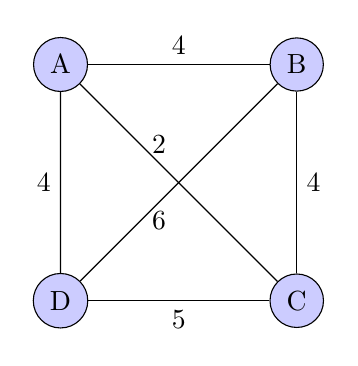
\begin{tikzpicture}[scale=3, every node/.style={circle, draw, fill=blue!20}]
			% Nodes
			\node (1) at (2,0) {D};
			\node (2) at (3,0) {C};
			\node (3) at (3,1) {B};
			\node (4) at (2,1) {A};
			% Edges with weights
			\draw (1) -- (2) node[midway, below, fill=none, draw=none, shape=rectangle] {$5$};
			\draw (2) -- (3) node[midway, right, fill=none, draw=none, shape=rectangle] {$4$};
			\draw (3) -- (4) node[midway, above, fill=none, draw=none, shape=rectangle] {$4$};
			\draw (4) -- (1) node[midway, left, fill=none, draw=none, shape=rectangle] {$4$};
			\draw (1) -- (3) node[pos = 0.4, below, fill=none, draw=none, shape=rectangle] {$6$};
			\draw (2) -- (4) node[pos = 0.6, above, fill=none, draw=none, shape=rectangle] {$2$};
		\end{tikzpicture}
	\end{center}
	
	\begin{equation*}
		w =  \{w_{AB},w_{AC},w_{AD},w_{BC},w_{CD},w_{BD}\} =  \{4,2,4,4,5,6\}
	\end{equation*}
	
	
	\subsection{Algorithm Construction}
	
	We will follow the instructions highlighted at the begining of chapter 3. We start by normalizing our edge weights. We need to sort our all edge weights in descending order as in equation \ref{sorted-weights}:	
	
	\begin{equation*}
	w' = \{6,5,4,4,4,2\}
	\end{equation*}
	
	
	Then we need to retrieve the sum $S$ as in equation \ref{sum-S}
	\begin{equation*}
	S = \sum_{i=1}^{4} w'_i = 6 + 5  + 4 + 4 = 19
	\end{equation*}
	
	From here we can normalize our edgeweights as in \ref{normalization}, we can set $\epsilon = 1$
	
	\begin{equation*}
		\tilde{w} = \frac{ \{4,2,4,4,5,6\}}{20} = \{0.2 , 0.1 , 0.2 , 0.2 , 0.25, 0.3\} 
	\end{equation*}
	
	
	
	
	\begin{center}	
		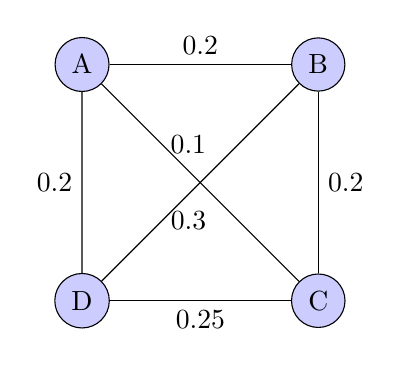
\begin{tikzpicture}[scale=3, every node/.style={circle, draw, fill=blue!20}]
			% Nodes
			\node (1) at (2,0) {D};
			\node (2) at (3,0) {C};
			\node (3) at (3,1) {B};
			\node (4) at (2,1) {A};
			% Edges with weights
			\draw (1) -- (2) node[midway, below, fill=none, draw=none, shape=rectangle] {$0.25$};
			\draw (2) -- (3) node[midway, right, fill=none, draw=none, shape=rectangle] {$0.2$};
			\draw (3) -- (4) node[midway, above, fill=none, draw=none, shape=rectangle] {$0.2$};
			\draw (4) -- (1) node[midway, left, fill=none, draw=none, shape=rectangle] {$0.2$};
			\draw (1) -- (3) node[pos = 0.4, below, xshift=1mm, fill=none, draw=none, shape=rectangle] {$0.3$};
			\draw (2) -- (4) node[pos = 0.6, above,xshift=1mm, fill=none, draw=none, shape=rectangle] {$0.1$};
		\end{tikzpicture}
	\end{center}
	
	
	Now we need to construct the unitary operator and eigenstates. Our matrix $U$ and $U'$ diagonals will look like the following:
	
	
	\begin{align*}	
		u & = \begin{bmatrix}
			1 \\
			e^{i2\pi(0.2)} \\
			e^{i2\pi(0.1)} \\
			e^{i2\pi(0.2)} \\
		\end{bmatrix} 
		\otimes \begin{bmatrix}
			e^{i2\pi(0.2)} \\
			1 \\
			e^{i2\pi(0.2)} \\
			e^{i2\pi(0.3)} \\
		\end{bmatrix}
		\otimes \begin{bmatrix}
			e^{i2\pi(0.1)} \\
			e^{i2\pi(0.2)} \\
			1\\
			e^{i2\pi(0.25)} \\
		\end{bmatrix} 
		\otimes \begin{bmatrix}
		e^{i2\pi(0.2)} \\
		e^{i2\pi(0.3)} \\
		e^{i2\pi(0.25)} \\
			1 \\
		\end{bmatrix} 						 			
	\end{align*}
	
	\begin{align*}	
		u' & = \begin{bmatrix}
			1 \\
			e^{i2\pi(0.2)} \\
			e^{i2\pi(0.1)} \\
			e^{i2\pi(0.2)} \\
		\end{bmatrix} 
		\otimes \begin{bmatrix}
			e^{i2\pi(0.2)} \\
			1 \\
			e^{i2\pi(0.2)} \\
			e^{i2\pi(0)} \\
		\end{bmatrix}
		\otimes \begin{bmatrix}
			e^{i2\pi(0.1)} \\
			e^{i2\pi(0.2)} \\
			1\\
			e^{i2\pi(0.25)} \\
		\end{bmatrix} 
		\otimes \begin{bmatrix}
			e^{i2\pi(0.2)} \\
			e^{i2\pi(0)} \\
			e^{i2\pi(0.25)} \\
			1 \\
		\end{bmatrix} 						 			
	\end{align*}
	
	
	Because we are dealing with the symmetric case. Based on Table \ref{table:ham-cycle-details-4-city} we can simply use the results and conversions from the first three cycles. Thus we will be estimating phases using the following eigenstates:
	
	$$|108\rangle = |01101100\rangle$$
	$$|114\rangle = |01110010\rangle$$
	$$|180\rangle = |10110100\rangle$$
	And expect the following phases:
	
	\vspace{1cm}
	Cycle 1: $A \rightarrow B \rightarrow C \rightarrow D \rightarrow A$
	
	\begin{center}	
		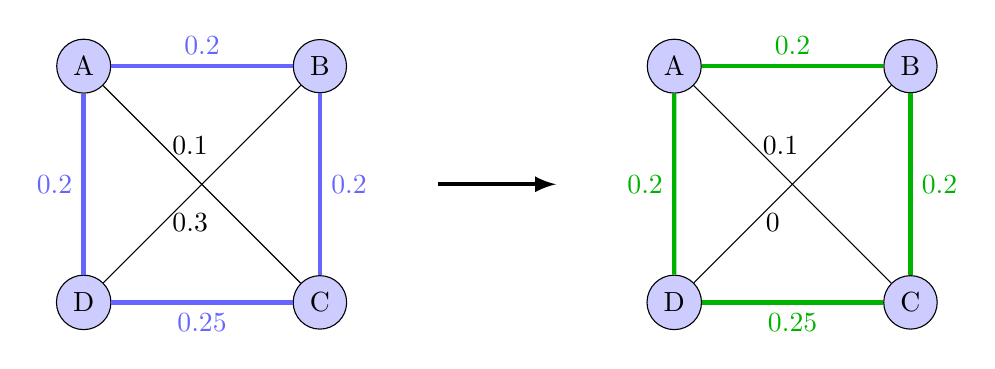
\begin{tikzpicture}[scale=3, every node/.style={circle, draw, fill=blue!20}]
			% Nodes
			\node (1) at (0,0) {D};
			\node (2) at (1,0) {C};
			\node (3) at (1,1) {B};
			\node (4) at (0,1) {A};
			% Edges with weights
			\draw[blue!60, ultra thick] (1) -- (2) node[midway, below, fill=none, draw=none, shape=rectangle] {$0.25$};
			\draw[blue!60,ultra  thick] (2) -- (3) node[midway, right, fill=none, draw=none, shape=rectangle] {$0.2$};
			\draw [blue!60, ultra thick](3) -- (4) node[midway, above, fill=none, draw=none, shape=rectangle] {$0.2$};
			\draw [blue!60,ultra  thick](4) -- (1) node[midway, left, fill=none, draw=none, shape=rectangle] {$0.2$};
			\draw (1) -- (3) node[pos = 0.4, xshift=1mm, below, fill=none, draw=none, shape=rectangle] {$0.3$};
			\draw (2) -- (4) node[pos = 0.6, xshift=1mm, above, fill=none, draw=none, shape=rectangle] {$0.1$};
			
			
			
			% Nodes
			\node (5) at (2.5,0) {D};
			\node (6) at (3.5,0) {C};
			\node (7) at (3.5,1) {B};
			\node (8) at (2.5,1) {A};
			% Edges with weights
			\draw[black!30!green, ultra thick] (5) -- (6) node[midway, below, fill=none, draw=none, shape=rectangle] {$0.25$};
			\draw[black!30!green, ultra thick] (6) -- (7) node[midway, right, fill=none, draw=none, shape=rectangle] {$0.2$};
			\draw [black!30!green, ultra thick](7) -- (8) node[midway, above, fill=none, draw=none, shape=rectangle] {$0.2$};
			\draw [black!30!green, ultra thick](8) -- (5) node[midway, left, fill=none, draw=none, shape=rectangle] {$0.2$};
			\draw (5) -- (7) node[pos = 0.4, below, fill=none, draw=none, shape=rectangle] {$0$};
			\draw (6) -- (8) node[pos = 0.6, xshift=1mm, above, fill=none, draw=none, shape=rectangle] {$0.1$};
			
			\draw[->, ultra thick, >=latex] (1.5, 0.5) -- (2, 0.5);
			
		\end{tikzpicture}
	\end{center}
	
	
	 $$u_{108} = e^{i2\pi (\gamma_{AB} + \gamma_{BC} + \gamma_{CD} + \gamma_{DA})} = e^{i2\pi(0.85)}$$
	 $$u'_{108} = e^{i2\pi (\gamma_{AB} + \gamma_{BC} + \gamma_{CD} + \gamma_{DA})} = e^{i2\pi(0.85)}$$
	 
	  \vspace{1cm}
	 
	 Cycle 2: $A \rightarrow B \rightarrow D \rightarrow C \rightarrow A$
	 
	 \begin{center}	
	 	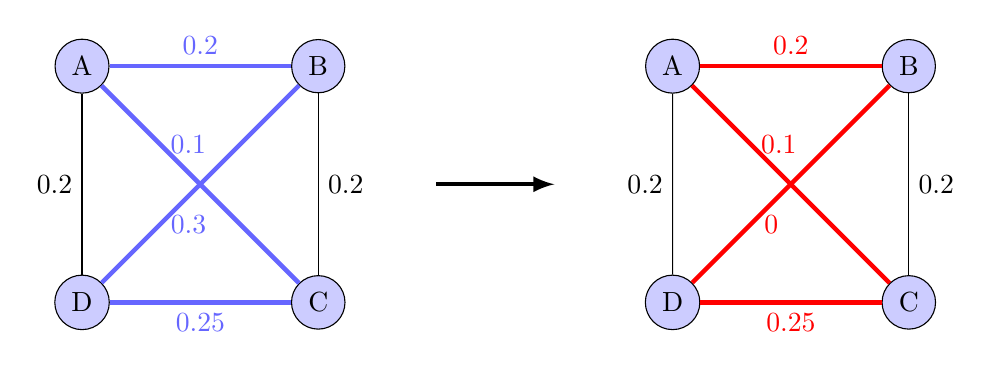
\begin{tikzpicture}[scale=3, every node/.style={circle, draw, fill=blue!20}]
	 		% Nodes
	 		\node (1) at (0,0) {D};
	 		\node (2) at (1,0) {C};
	 		\node (3) at (1,1) {B};
	 		\node (4) at (0,1) {A};
	 		% Edges with weights
	 		\draw [blue!60, ultra thick](1) -- (2) node[midway, below, fill=none, draw=none, shape=rectangle] {$0.25$};
	 		\draw (2) -- (3) node[midway, right, fill=none, draw=none, shape=rectangle] {$0.2$};
	 		\draw [blue!60, ultra thick](3) -- (4) node[midway, above, fill=none, draw=none, shape=rectangle] {$0.2$};
	 		\draw (4) -- (1) node[midway, left, fill=none, draw=none, shape=rectangle] {$0.2$};
	 		\draw [blue!60, ultra thick](1) -- (3) node[pos = 0.4, xshift=1mm, below, fill=none, draw=none, shape=rectangle] {$0.3$};
	 		\draw [blue!60, ultra thick](2) -- (4) node[pos = 0.6, xshift=1mm, above, fill=none, draw=none, shape=rectangle] {$0.1$};
	 		
	 		
	 		
	 		% Nodes
	 		\node (5) at (2.5,0) {D};
	 		\node (6) at (3.5,0) {C};
	 		\node (7) at (3.5,1) {B};
	 		\node (8) at (2.5,1) {A};
	 		% Edges with weights
	 		\draw[red, ultra thick] (5) -- (6) node[midway, below, fill=none, draw=none, shape=rectangle] {$0.25$};
	 		\draw (6) -- (7) node[midway, right, fill=none, draw=none, shape=rectangle] {$0.2$};
	 		\draw [red, ultra thick](7) -- (8) node[midway, above, fill=none, draw=none, shape=rectangle] {$0.2$};
	 		\draw (8) -- (5) node[midway, left, fill=none, draw=none, shape=rectangle] {$0.2$};
	 		\draw  [red, ultra thick](5) -- (7) node[pos = 0.4, below, fill=none, draw=none, shape=rectangle] {$0$};
	 		\draw  [red,ultra  thick](6) -- (8) node[pos = 0.6, xshift=1mm, above, fill=none, draw=none, shape=rectangle] {$0.1$};
	 		
	 		\draw[->, ultra thick, >=latex] (1.5, 0.5) -- (2, 0.5);
	 		
	 	\end{tikzpicture}
	 \end{center}
	 
	 $$ u_{114} = e^{i2\pi (\gamma_{AB} + \gamma_{BD} + \gamma_{DC} + \gamma_{CA})} = e^{i2\pi(0.85)}$$
	 $$ u'_{114} = e^{i2\pi (\gamma_{AB} + \gamma_{BD} + \gamma_{DC} + \gamma_{CA})} = e^{i2\pi(0.55)}$$
	 
	 \vspace{1cm}
	 
	 Cycle 3: $A \rightarrow C \rightarrow B \rightarrow D \rightarrow A$
	 
	 \begin{center}	
	 	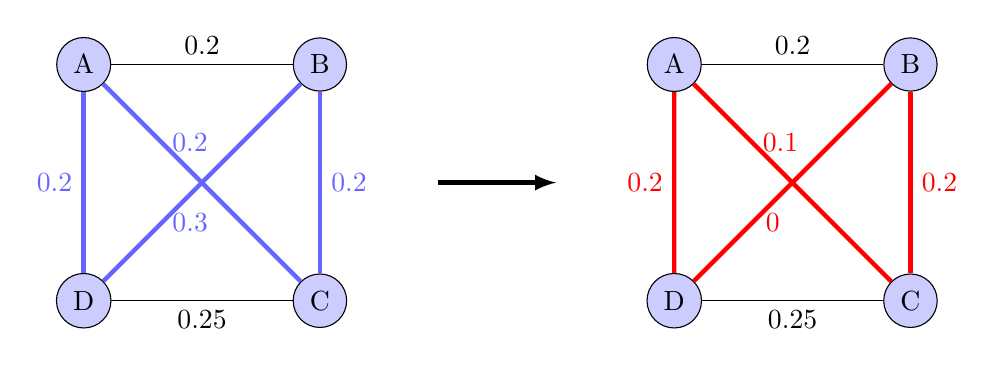
\begin{tikzpicture}[scale=3, every node/.style={circle, draw, fill=blue!20}]
	 		% Nodes
	 		\node (1) at (0,0) {D};
	 		\node (2) at (1,0) {C};
	 		\node (3) at (1,1) {B};
	 		\node (4) at (0,1) {A};
	 		% Edges with weights
	 		\draw (1) -- (2) node[midway, below, fill=none, draw=none, shape=rectangle] {$0.25$};
	 		\draw [blue!60, ultra thick](2) -- (3) node[midway, right, fill=none, draw=none, shape=rectangle] {$0.2$};
	 		\draw (3) -- (4) node[midway, above, fill=none, draw=none, shape=rectangle] {$0.2$};
	 		\draw [blue!60,ultra thick](4) -- (1) node[midway, left, fill=none, draw=none, shape=rectangle] {$0.2$};
	 		\draw [blue!60,ultra thick](1) -- (3) node[pos = 0.4, xshift=1mm, below, fill=none, draw=none, shape=rectangle] {$0.3$};
	 		\draw [blue!60,ultra thick](2) -- (4) node[pos = 0.6, xshift=1mm, above, fill=none, draw=none, shape=rectangle] {$0.2$};
	 		
	 		% Nodes
	 		\node (5) at (2.5,0) {D};
	 		\node (6) at (3.5,0) {C};
	 		\node (7) at (3.5,1) {B};
	 		\node (8) at (2.5,1) {A};
	 		% Edges with weights
	 		\draw (5) -- (6) node[midway, below, fill=none, draw=none, shape=rectangle] {$0.25$};
	 		\draw [red,ultra thick](6) -- (7) node[midway, right, fill=none, draw=none, shape=rectangle] {$0.2$};
	 		\draw (7) -- (8) node[midway, above, fill=none, draw=none, shape=rectangle] {$0.2$};
	 		\draw [red,ultra thick](8) -- (5) node[midway, left, fill=none, draw=none, shape=rectangle] {$0.2$};
	 		\draw  [red,ultra thick](5) -- (7) node[pos = 0.4, below, fill=none, draw=none, shape=rectangle] {$0$};
	 		\draw  [red,ultra thick](6) -- (8) node[pos = 0.6, xshift=1mm, above, fill=none, draw=none, shape=rectangle] {$0.1$};
	 		
	 		% Arrow pointing from the first graph to the second graph
	 		\draw[->, ultra thick, >=latex] (1.5, 0.5) -- (2, 0.5);% node[midway, above,  fill=none, draw=none, shape=rectangle] {Transition};
	 		
	 	\end{tikzpicture}
	 \end{center}
	 
	 $$ u_{180} = e^{i2\pi (\gamma_{AC} + \gamma_{CB} + \gamma_{BD} + \gamma_{DA})} = e^{i2\pi(0.80)}$$
	$$ u'_{180} = e^{i2\pi (\gamma_{AC} + \gamma_{CB} + \gamma_{BD} + \gamma_{DA})} = e^{i2\pi(0.50)}$$
	
	\subsection{Results: Simulations with Qiskit}
	
	The basis of our algorithm is to perform phase estimation before and after the edgeweights that do not satify the criteria above are removed. Below we highlight each hamiltonian cycles before and after the criteria. If the hamiltonian cycle is not affected we highlight in green vs red.




\vspace{0.5cm}






		\begin{figure}[!h]
		\centering
		\includegraphics[trim={8.5cm 4.4cm 6cm 4.4cm},clip, width=1 \linewidth]{"graphics/4-city-1-cycle-constrained-barrier"}
		\caption{the quantum circuit for the BTSP: 3 qubit phase estimation is performed measuring the hamiltonian cycle $A \rightarrow B \rightarrow C \rightarrow D \rightarrow A$, using the corresponding eigenstate is $|01101100\rangle$. Due to Qiskit convention on qubit ordering, the eigentate is initialized in reverse. The CU gate denotes the control unitary matrix containing all the hamiltonian cycles. The CU' gate inhabits the same cycles but before it was constructed, all edgeweights not satisfying the constraint, $\geq \alpha$, were set to zero. We have two sets of 3 qubits to be measured and stored in to classical registers labelled 'output' and 'output c'.}
		\label{fig:4-city-graphic}
	\end{figure}		


	\begin{figure}[!h]
		\centering
		\includegraphics[width=\textwidth,height=0.9\textheight,keepaspectratio]{"graphics/3qubit-4city"}
		\caption{3-qubit phase estimation for the 4-city problem}
		\label{fig:4-city-graphic}
	\end{figure}		
	
		\begin{figure}[!h]
		\centering
		\includegraphics[ width=\textwidth,height=0.9\textheight,keepaspectratio]{"graphics/4qubit-4city"}
		\caption{4-qubit phase estimation for the 4-city problem}
		\label{fig:4-city-graphic}
	\end{figure}		
	
		\begin{figure}[!h]
		\centering
		\includegraphics[width=\textwidth,height=0.9\textheight,keepaspectratio]{"graphics/5qubit-4city"}
		\caption{5-qubit phase estimation for the 4-city problem}
		\label{fig:4-city-graphic}
	\end{figure}		
	

	\section{An Undirected 5-City Graph}
	
	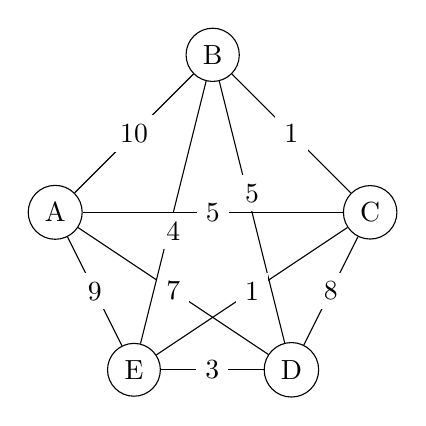
\begin{tikzpicture}[scale=1, every node/.style={circle,draw}]
	\node (A) at (0, 2) {A};
	\node (B) at (2, 4) {B};
	\node (C) at (4, 2) {C};
	\node (D) at (3, 0) {D};
	\node (E) at (1, 0) {E};
	\draw (A) -- (B) node[midway, fill=white, draw=none, shape=rectangle] {10};
	\draw (A) -- (C) node[midway, fill=white, draw=none, shape=rectangle] {5};
	\draw (A) -- (D) node[midway, fill=white, draw=none, shape=rectangle] {7};
	\draw (A) -- (E) node[midway, fill=white, draw=none, shape=rectangle] {9};
	\draw (B) -- (C) node[midway, fill=white, draw=none, shape=rectangle] {1};
	\draw (B) -- (D) node[midway,above,  fill=white, draw=none, shape=rectangle] {5};
	\draw (B) -- (E) node[midway, below,fill=white, draw=none, shape=rectangle] {4};
	\draw (C) -- (D) node[midway, fill=white, draw=none, shape=rectangle] {8};
	\draw (C) -- (E) node[midway, fill=white, draw=none, shape=rectangle] {1};
	\draw (D) -- (E) node[midway,fill=white, draw=none, shape=rectangle] {3};
	
	\end{tikzpicture}

	
	\vspace{0.5cm}
	
	
	
	%\section{Tables}
We have already included one table:~\ref{tab:Table1}.  Another table
is plopped right here.
\begin{table}[ht]
  \begin{center}
    \begin{tabular}{|l||l|l||l|l|}
      \hline
      &\multicolumn{2}{l|}{Singular}&\multicolumn{2}{l|}{Plural}\\
      \cline{2-5}
       &English&\textbf{Gaeilge}&English&\textbf{Gaeilge}\\
      \hline\hline
      1st Person&at me&\textbf{agam}&at us&\textbf{againn}\\
      2nd Person&at you&\textbf{agat}&at you&\textbf{agaibh}\\
      3rd Person&at him&\textbf{aige}&at them&\textbf{acu}\\
       &at her&\textbf{aici}& & \\
      \hline
    \end{tabular}
    \caption{
      \label{tab:Table2}
      Another table.}
  \end{center}
\end{table}
	%\input{Results/RSLT02}
	\chapter{Discussion}
	%\input{Discussion/DISC01}
	
	\begin{enumerate}
		\item this section will dicuss the advantages and drawbacks of the algorithm proposed.
		\item how the algorithm scales with the number of cities ($2^x = x^x$)
	\end{enumerate}
	
	
	%% This file is setup to use a bibtex file sample.bib and uses the
	%% plain style.  Other styles may be used depending on the conventions
	%% of your field of study.
	%%
	%%% Note: the bibliography must come before the appendices.
	% \bibliographystyle{JHEP}
	% \bibliographystyle{plainnat}
	\bibliographystyle{unsrt}
	%\bibliography{references,refs}
	\bibliography{ref}
	%\printbibliography  %[heading=none, keyword=OWN]
	%% Use this to reset the appendix counter.  Note that the FoGS
	%% requires that the word ``Appendices'' appear in the table of
	%% contents either before each appendix lable or as a division
	%% denoting the start of the appendices.  We take the latter option
	%% here.  This is ensured by making the \texttt{appendicestoc} option
	%% a default option to the UBC thesis class.
	
	%%% If you only have one appendix, please uncomment the following line.
	% \renewcommand{\appendicesname}{Appendix}
	\appendix
	\chapter{Code: Calculating the Hamiltonian Cycles and Locating Eigenstates}
	
	\includepdf[pages=-]{hamiltonian_cycles.pdf}
	%\input{ham_cycles.tex}
	%\input{hamiltonian_cycles.tex}
	\chapter{Code: 4-City Problem}
	
	\includepdf[pages=-]{4-city-code/4-city-code.pdf}
	
	\chapter{Code: 5-city constraint problem}
	
	\begin{enumerate}
		\item this section will include any code used to produce graphs in the simulated section.
	\end{enumerate}
	
	
	%In this appendix, I show that the spherical Morlet wavelet introduced in \cref{sec:ST} satisfies all wavelet requirements. 
There are three conditions for a wavelet:

\begin{enumerate}
    \item translation invariant 
    \item localized in both real space and Fourier space 
    \item wavelet should be admissible 
    \begin{equation}
        c_{\psi} \equiv (2 \pi)^2 \int_{\mathbb{R}^2} \frac{|\widetilde{\psi}(k)|^{2}}{|k|^2} d k<\infty
    \end{equation}
        which essentially gives a weaker admissibility condition
        \begin{equation}
            \widetilde{\psi}(0) = 0
        \end{equation}

    
\end{enumerate}
	
	%\chapter{Second Appendix}
	%Here is the second appendix.
	
	%% This changes the headings and chapter titles (no numbers for
	%% example).
	\backmatter
	
	%% Indices come here if you have them.
	
	
	
	
	
	
	
	
	%\url{http://www.grad.ubc.ca/current-students/dissertation-thesis-preparation}\\
	
	
	\end{document}
	
	
	
\end{document}
